% =====================================================================
% A Single Chain Suffices: Re-examining Diversity-Enhanced flowMC
% Ensembles under Equal Sampling Budgets  --  REVISED VERSION
%
% Standalone article-class source. Compiles with pdflatex out of the box
% (pdflatex main.tex, twice for cross-references).
% For journal submission, paste the body into the target template.
% Table bodies are generated from the released CSVs by code/gen_tables.py
% and live in tables/; figures live in figures/.
% =====================================================================
\documentclass[11pt]{article}

\usepackage[utf8]{inputenc}
\usepackage[T1]{fontenc}
\usepackage{amsmath,amssymb}
\usepackage{graphicx}
\usepackage{booktabs}
\usepackage{authblk}
\usepackage[margin=1in]{geometry}
\usepackage{caption}
\usepackage[hidelinks]{hyperref}

\graphicspath{{figures/}}

\title{\textbf{A Single Chain Suffices: Re-examining Diversity-Enhanced
flowMC Ensembles under Equal Sampling Budgets}}
\author[1]{Mingyu Shi}
\affil[1]{Independent Researcher}
\date{}

\begin{document}
\maketitle

\begin{abstract}
\noindent
Normalizing-flow Markov chain Monte Carlo (MCMC), of which flowMC [1,2] is a
representative implementation, adds a learned global proposal on top of local
moves. This paper began as an attempt to validate a natural reliability idea
--- run several such samplers with different architectures and pool their
samples: a five-member diverse flowMC ensemble equipped with
three aggregation mechanisms --- ESS-based adaptive tempering, coverage-aware
reweighting, and quality-based member weighting. On six benchmark targets in
20 and 50 dimensions, the ensemble seemed to reduce the average marginal
Jensen--Shannon (JS) distance by about 18\% relative to a single flowMC chain,
significantly on every configuration. One control reversed the story: the
ensemble draws five times as many samples as the baseline (10{,}000 against
2{,}000), and histogram-based JS distance carries a finite-sample bias. At a
matched 10{,}000-sample budget, a single chain beats the ensemble on nine of
eleven configurations, ties on the other two, lowers the mean JS by a further
24\%, and runs about six times faster. We show that the JS estimate of a
perfect sampler follows the closed form $\sqrt{c\,(1/N+1/M)}$ with
$c\approx(B_{\mathrm{eff}}-1)/8$ nats, which explains the original ``gain''
almost entirely. We then reproduce the ensemble's deficit \emph{without
running flowMC at all}: applying the released aggregation operators to exact
draws from the targets recovers about 90\% of the gap, and adding the
tempering schedule reproduces the measured ensemble values. The damage decomposes into a genuine distribution shift
caused by the coverage and tempering reweighting --- confirmed by an unbiased
energy distance --- and a pure estimator-level loss caused by resampling with
replacement, which halves the effective histogram sample. Uniform pooling is
harmless and matches the single chain, and adding members (up to twenty) does
not repair the aggregation. On real Bayesian posteriors, scored against a long
NUTS reference with unbiased joint metrics (energy distance and $\mathrm{MMD}^2$)
as well as marginal JS, uniform pooling is closest to the true posterior on
every run, while the ensemble's disadvantage proves specific to the biased
marginal metric --- a reversal the finite-sample analysis predicts. An audit of
the reference generators shows that two synthetic targets were scored against
a law that differs from their potential. The recommendation is unchanged and now
mechanistic: run one flowMC chain at the full budget; if members are pooled,
pool them uniformly; and be aware that reweight-and-resample aggregation harms
the marginal fit even where its effect on the joint posterior is small.
\end{abstract}

\noindent\textbf{Keywords:} Markov chain Monte Carlo; normalizing flows;
ensemble sampling; negative results; Jensen--Shannon divergence;
finite-sample bias; divergence estimation

\section{Introduction}

Sampling from complex, high-dimensional and multimodal distributions is one
of the recurring difficulties in Bayesian inference [5]. Normalizing-flow
MCMC, such as flowMC [1,2], combines local gradient-based moves with a global
proposal drawn from a normalizing flow [3,4] that is trained on the running
samples. On targets where purely local samplers move slowly, this kind of
method usually does well.

When we began this work, our reasoning was the common one: if a single
flow-based sampler is good, then a group of them, built with different flow
architectures and different step budgets, should be even more reliable,
because the weak points of one member could be covered by the others.
Ensemble and population MCMC have a long tradition along this line [6,7,8]. So
we designed a diverse five-member flowMC ensemble and added three lightweight
aggregation mechanisms, each aimed at a failure mode we expected: adaptive
tempering for members that explore poorly, coverage-aware reweighting for
regions that get missed, and quality-based member weighting so that weaker
members count less.

At first the results agreed with our expectation. Across six targets in 20
and 50 dimensions, the ensemble lowered the average marginal JS distance to a
reference sample by about 18\% relative to a single chain, and on every
configuration the difference was statistically significant. We were ready to
write this up as a positive method.

The reason this paper is a negative result instead is one control experiment.
With the budget allocation we used, called equal-per-member, every member
draws as many samples as the single-chain baseline, so five members produce
five times the samples in total --- 10{,}000 against 2{,}000. Histogram-based
JS distance is not a fair quantity to compare across different sample sizes,
because it carries an upward bias that shrinks as the number of samples grows.
The honest comparison is therefore not a single chain at 2{,}000 samples, but
a single chain at the same total of 10{,}000.

We ran it, and it reversed the conclusion. A single flowMC chain at 10{,}000
samples is better than the ensemble on nine of eleven configurations, ties on
the two remaining ones, and lowers the mean JS by a further 24\%. The ensemble
never wins. We then checked the metric itself by drawing directly from the
true distributions, and found that even a perfect sampler's marginal JS
estimate moves from about 0.085 at 2{,}000 samples to about 0.043 at 10{,}000
--- a factor close to two, and almost the same number for every target. A
second-order analysis of the estimator (Section~\ref{sec:why}) shows why: the
squared JS estimate of a perfect sampler is linear in $1/N+1/M$ with a slope
set by the number of histogram bins, so the floor is a property of the metric,
not of the target. This accounts for the original ``gain'' on its own.

After that, we kept digging, and the ensemble came apart piece by piece. A
homogeneous ensemble of five identical members performs the same as the
diverse one, so diversity does nothing here. None of the three aggregation
mechanisms helps in the ablation; two of them slightly hurt. When we throw
away the aggregation step entirely and simply concatenate the members' raw
samples, the accuracy returns to the single-chain level. Finally --- and this
is the part that turns the negative result into an explanation --- we removed
flowMC itself: we applied the released aggregation operators to \emph{exact}
draws from the targets, and the deficit reappeared almost unchanged. About
90\% of the gap between the ensemble and the matched single chain is
reproduced by the aggregation acting on perfect samples, and adding the
adaptive-tempering schedule reproduces the measured ensemble values on the
correlated and funnel targets to within a few thousandths. The mechanism
splits cleanly in two: the coverage and tempering reweighting genuinely
distorts the sampled distribution (an unbiased energy distance confirms the
shift), while the resampling-with-replacement step leaves the distribution
intact but duplicates points, which halves the effective sample behind the
histogram and pushes the biased JS estimator upward. Pooling the members is
harmless; every part of the machinery we put around the pooling either
distorts the law or degrades the estimate.

We think this is worth reporting, precisely because the positive version of
the story is the easy one to believe and the easy one to publish. The single
experiment that breaks it is cheap. The contributions of this paper are:

\begin{enumerate}
\item We show that the apparent advantage of a diversity-enhanced flowMC
ensemble over a single chain is, for these targets and budgets, an artifact of
comparing at unequal sample counts, and we give the closed-form finite-sample
law of the metric, $\mathbb{E}[\widehat{\mathrm{JS}}^{\,2}]\approx
c\,(1/N+1/M)$ with $c\approx(B_{\mathrm{eff}}-1)/8$ nats, that quantifies the
artifact and is verified across sample sizes and bin counts.
\item With a matched-budget control, a single chain matches or beats the
ensemble on every configuration (better on nine of eleven, tied on the two
banana cases) and is also about six times faster; plain uniform pooling of the
members recovers single-chain accuracy, which localizes the entire deficit in
the aggregation step.
\item We reproduce and decompose the deficit \emph{without flowMC}: the
released aggregation operators applied to exact draws recover about 90\% of
the gap, and with the tempering schedule they reproduce the measured ensemble
on the correlated and funnel targets. The decomposition separates a genuine
distribution shift (coverage and tempering reweighting; confirmed under an
unbiased energy distance) from a pure estimator-level loss (resampling with
replacement, which doubles the sampler-side variance term exactly as the
bootstrap predicts). Increasing the ensemble size to twenty members does not
repair the aggregation.
\item We confirm the conclusions on \emph{real posteriors} with the \emph{real
sampler} and \emph{unbiased joint metrics}, closing the two objections that the
synthetic marginal-JS study leaves open. On Bayesian logistic-regression and
hierarchical-model posteriors, scored against a long NUTS reference, the uniform
pool is closest to the true posterior under the energy distance, $\mathrm{MMD}^2$
and marginal JS on all fifteen target--metric--repetition runs; the single chain
still beats the full ensemble on marginal JS; and the full ensemble is often
best under the unbiased joint metrics --- a metric-specific reversal that the
finite-sample-bias analysis predicts and that turns a potential inconsistency
into corroboration of the paper's central point.
\item We document two practical methodological warnings: histogram-based
divergences are only comparable at matched sample counts and should be
reported together with their finite-sample floor; and reference generators
must be validated against the potential --- an audit shows that for two of our
six targets the released reference law differs from the law defined by the
potential, which changes the interpretation of which targets are
sampler-limited.
\end{enumerate}

\section{Background and Related Work}

\subsection{Normalizing-flow MCMC}
A normalizing flow writes a distribution as an invertible, learnable
transformation of a simple base density, with a tractable Jacobian [3,4].
flowMC [1,2] uses such a flow as a global independence proposal together with
local Metropolis-adjusted Langevin steps, and trains a rational-quadratic
neural spline flow [4] in alternating training and production phases. In this
work we keep flowMC unchanged both for the single-chain baseline and for each
ensemble member, so that any difference we see comes from ensembling and
aggregation, not from a modified kernel.

\subsection{Ensemble and population MCMC}
Combining several chains to gain reliability is an old idea, including
affine-invariant ensemble samplers [6] and their popular implementation [7],
as well as population-based and tempering methods more generally [8,9]. Our
setup is different in one respect: the members do not talk to each other while
sampling. They are independent flowMC runs and are combined only at the
aggregation stage. This isolates the effect of pooling several members from
any inter-chain communication.

\subsection{Evaluating sample quality}
We measure the marginal JS distance [11] between the sampler output and a
large reference sample, averaged over the dimensions, together with effective
sample size [12] and runtime. A point that becomes central later
(Section~\ref{sec:why}) is that histogram-based divergence estimators carry a
positive finite-sample bias of the same origin as the classical bias of
plug-in entropy estimates [14,15], so a comparison made at different sample
counts can mislead. We also use the energy distance [16], whose unbiased
U-statistic form has expectation zero when the two samples follow the same
law, as a joint-distribution check that is free of this bias; kernel
two-sample statistics such as MMD [17] would serve the same purpose.

\section{Methods}

\subsection{Single flowMC baseline}
The baseline is one flowMC sampler with two training and two production loops,
ten local MALA steps and ten global flow steps per loop, and five training
epochs per loop. The flow is a rational-quadratic spline with three coupling
layers, eight bins, and two hidden layers of width 64. These settings are kept
fixed across all targets. We run this baseline at two sample sizes: 2{,}000
particles, which was our original baseline, and 10{,}000 particles, which is
the matched control whose total equals the ensemble. We call this single
flowMC run the ``single-chain'' baseline, following MCMC terminology, although
each run returns a set of particles rather than one sequential chain.

\subsection{Diverse ensemble}
The ensemble has five flowMC members that differ in capacity and step
allocation: hidden-layer widths
$((64,64),(96,96),(128,64),(64,128),(32,64,32))$, number of spline layers
(three or four), number of bins (eight to twelve), and the split between local
and global steps. The members are independent and are combined only at the
aggregation step.

\subsection{Aggregation mechanisms}
\label{sec:mechanisms}
Three mechanisms act at the aggregation stage. \textbf{Adaptive tempering}
changes a per-member temperature $T$ in
$\log\pi_T(x)=\tfrac{1}{T}\log\pi(x)$: after each member, $T$ is multiplied by
1.1 (capped at 2) if that member's ESS ratio falls below a target of 0.5, and
by 0.95 (floored at 0.1) otherwise, starting from $T=1$.
\textbf{Coverage-aware reweighting} clusters the pooled samples on their first
two coordinates with $k$-means ($K=8$, five initializations) and gives
inverse-frequency weights $w_i\propto 1/\mathrm{count}(c_i)$, followed by a
rare-cluster boost $w \leftarrow w\,(1+0.35\,(w/\max w - 1))$.
\textbf{Quality-based member weighting} scores members by
\begin{equation}
s_m=\mathrm{ESS}_m^{\beta}\,\exp(-\gamma\,\mathrm{JS}_m)\,
\exp(-\lambda\,\sigma_{\log p,m}),
\label{eq:score}
\end{equation}
with $\beta=1$, $\gamma=2$ and $\lambda=0.05$, standardizes the scores, and
turns them into weights with a softmax at temperature $\alpha=0.35$. Each
mechanism was chosen because it targeted a failure mode we believed mattered.
As Sections~\ref{sec:ablation} and~\ref{sec:decomp} report, none of them earns
its place.

\subsection{Pooling and budget allocation}
The pooled samples are combined by multiplying the member weights and the
coverage weights, normalizing, and \textbf{resampling with replacement} to a
target count of (per-member size) $\times$ (number of members). Under
\textbf{equal-per-member}, each member draws 2{,}000 samples, so the ensemble
total is 10{,}000. Under \textbf{equal-total}, the 2{,}000-sample budget is
split across members (400 each). The equal-per-member ensemble therefore uses
five times the compute and produces five times the samples of the
2{,}000-particle single chain, and the fair comparison is the
10{,}000-particle single chain.
Figure~\ref{fig:pipeline} summarizes the members, the tempering schedule, the
aggregation stack, and the two controls that the rest of the paper compares.

\begin{figure}[ht]
\centering
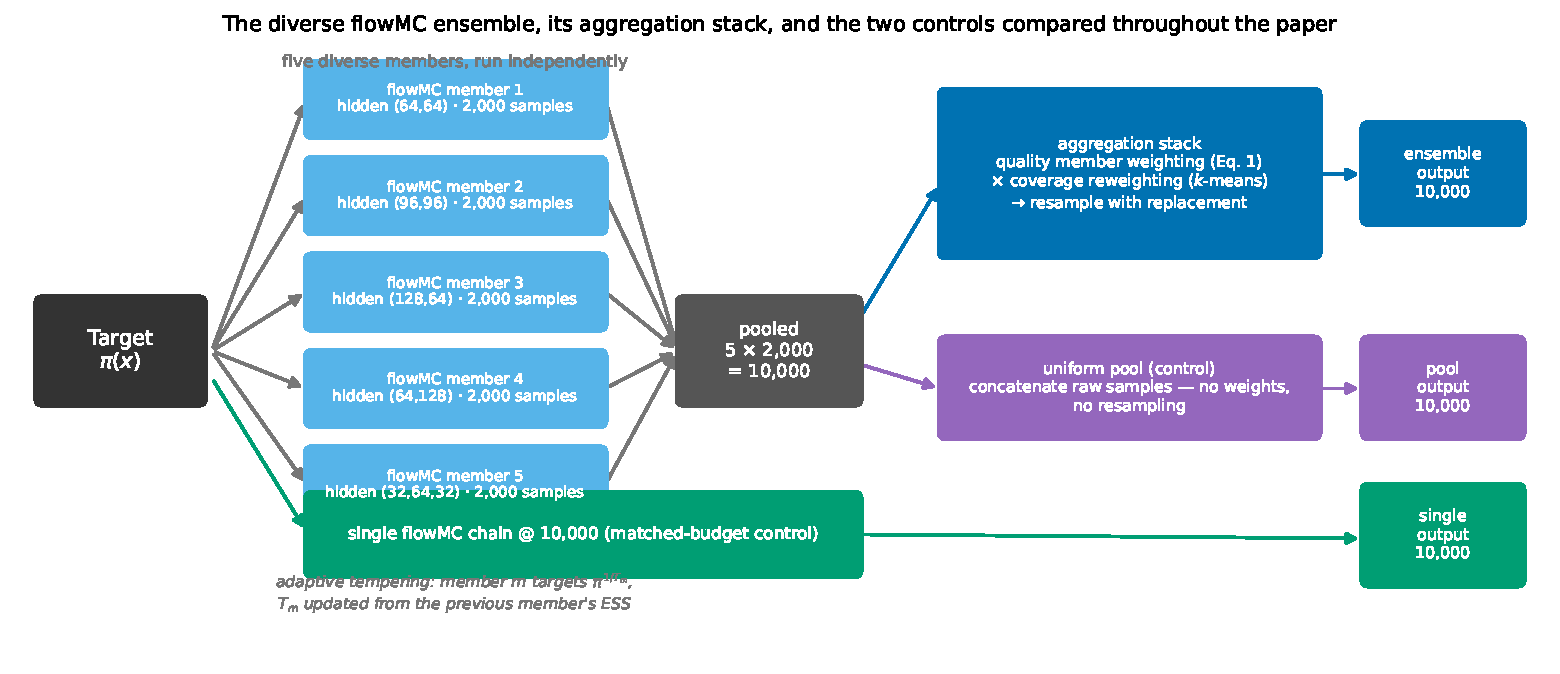
\includegraphics[width=\textwidth]{figures/fig_pipeline.pdf}
\caption{The pipeline under study. Five architecturally diverse flowMC members
(each targeting a tempered $\pi^{1/T_m}$ under the adaptive schedule) draw
2{,}000 samples each; the pooled 10{,}000 samples are then passed either
through the full aggregation stack (member weighting $\times$ coverage
reweighting, followed by resampling with replacement; blue) or through plain
uniform concatenation (purple). A single flowMC chain at the same
10{,}000-sample budget (green) is the matched-budget control.}
\label{fig:pipeline}
\end{figure}

\section{Experimental Setup}

\subsection{Targets and protocol}
We use six targets that stress different weaknesses of a sampler: a banana
density (strong nonlinear correlation), a bimodal Gaussian (separated modes),
Neal's funnel [10] (varying scale), a correlated Gaussian (correlation 0.95),
the Rosenbrock density (curved valley), and a Gaussian ring (eight modes on a
ring). All are run in 20 and 50 dimensions except the ring, which is 20D only,
giving eleven configurations. Each one is repeated five times with
deterministic seeds, the single-chain and ensemble runs in a repetition share
a seed stream, and the reference samples (20{,}000 per target) are drawn from
the generative form of each target. Section~\ref{sec:audit} audits these
reference generators against the potentials. All seeds, configurations and
code are released [13].

\subsection{Metrics}
The main metric is the average marginal JS distance computed on 100-bin
histograms whose range per dimension is the 0.5--99.5 percentile span of the
two samples, padded by 10\%. We also report ESS from the integrated
autocorrelation and the wall-clock runtime. The ESS we report is computed on
the returned particle or pooled sample array and serves only as a diagnostic
of duplication and correlation in the returned sample set; it should not be
read as a full trajectory-based MCMC mixing ESS. Where useful we give paired
$t$-tests and Cohen's $d$ over the five repetitions; tables report means $\pm$
one standard deviation over the repetitions.

\section{Results}

\subsection{The apparent ensemble gain}
\label{sec:apparent}
Against the 2{,}000-particle single chain, the equal-per-member ensemble
lowers the marginal JS distance on all eleven configurations, by 6.8\% to
29.2\% (mean 18.2\%), and every configuration is significant at $p<0.05$. Read
on its own, this looks like a clear success for ensembling, and the largest
improvements are on the multimodal and structured targets. The rest of this
section explains why it is not what it looks like.

\subsection{The equal-budget control}
\label{sec:control}
The equal-per-member ensemble draws 10{,}000 samples in total, while the
baseline it was compared with draws only 2{,}000. The fair comparison is a
single chain at 10{,}000 samples, which we give in Table~\ref{tab:control} and
Figure~\ref{fig:control}. The single 10{,}000-particle chain reaches a mean JS
of 0.065, against 0.085 for the ensemble and 0.104 for the 2{,}000-particle
baseline. It beats the ensemble on nine of eleven configurations, ties on the
two banana cases (within repetition noise), with 17\% to 44\% improvements on
exactly those targets where the ensemble had looked strongest (bimodal,
funnel, correlated, ring).

The single-chain advantage is not marginal where it exists: the
per-configuration gap is several to over a hundred times the single-chain
repetition standard deviation. The two banana cases are the exception, and
they are informative rather than awkward. There, both the single chain and the
ensemble sit far above the noise floor (JS around 0.10--0.14 against a floor
of 0.043), which tells us that flowMC is simply failing to capture the
banana's strong nonlinear correlation, no matter the sample count or the
ensembling. This is a sampler-limited regime, not a sample-limited one, and
the near-tie reflects that neither extra samples nor extra members help. So
the banana is not a case where ensembling succeeds; it is a case where nothing
we tried does. (The Rosenbrock and ring residuals above the floor turn out to
have a different explanation; see Section~\ref{sec:audit}.)

\begin{table}[htbp]
\centering
\caption{Marginal JS distance (mean $\pm$ sd over five repetitions). The
equal-budget single chain on the right is the proper control for the ensemble
in the middle. Lower is better. ``Tie'' marks differences within repetition
noise.}
\label{tab:control}
\small
\begin{tabular}{llcccc}
\toprule
Target & Dim & Single @2{,}000 & Ensemble @10{,}000 & Single @10{,}000 & Single@10k vs ens \\
\midrule
Banana & 20 & 0.169 $\pm$ 0.005 & 0.138 $\pm$ 0.004 & 0.137 $\pm$ 0.005 & tie \\
Banana & 50 & 0.127 $\pm$ 0.003 & 0.095 $\pm$ 0.003 & 0.097 $\pm$ 0.007 & tie \\
Bimodal & 20 & 0.087 $\pm$ 0.002 & 0.061 $\pm$ 0.001 & 0.045 $\pm$ 0.002 & $-27\%$ \\
Bimodal & 50 & 0.086 $\pm$ 0.001 & 0.061 $\pm$ 0.000 & 0.045 $\pm$ 0.001 & $-27\%$ \\
Correlated & 20 & 0.087 $\pm$ 0.001 & 0.081 $\pm$ 0.002 & 0.045 $\pm$ 0.001 & $-44\%$ \\
Correlated & 50 & 0.086 $\pm$ 0.001 & 0.071 $\pm$ 0.001 & 0.044 $\pm$ 0.000 & $-38\%$ \\
Funnel & 20 & 0.086 $\pm$ 0.002 & 0.074 $\pm$ 0.002 & 0.044 $\pm$ 0.000 & $-40\%$ \\
Funnel & 50 & 0.087 $\pm$ 0.001 & 0.079 $\pm$ 0.001 & 0.045 $\pm$ 0.000 & $-43\%$ \\
Ring & 20 & 0.097 $\pm$ 0.001 & 0.071 $\pm$ 0.001 & 0.059 $\pm$ 0.002 & $-17\%$ \\
Rosenbrock & 20 & 0.129 $\pm$ 0.001 & 0.114 $\pm$ 0.003 & 0.090 $\pm$ 0.001 & $-20\%$ \\
Rosenbrock & 50 & 0.103 $\pm$ 0.001 & 0.089 $\pm$ 0.001 & 0.062 $\pm$ 0.000 & $-30\%$ \\
\midrule
\textbf{Mean} & & \textbf{0.104} & \textbf{0.085} & \textbf{0.065} & \textbf{$-24\%$} \\
\bottomrule
\end{tabular}

\end{table}

\begin{figure}[htbp]
\centering
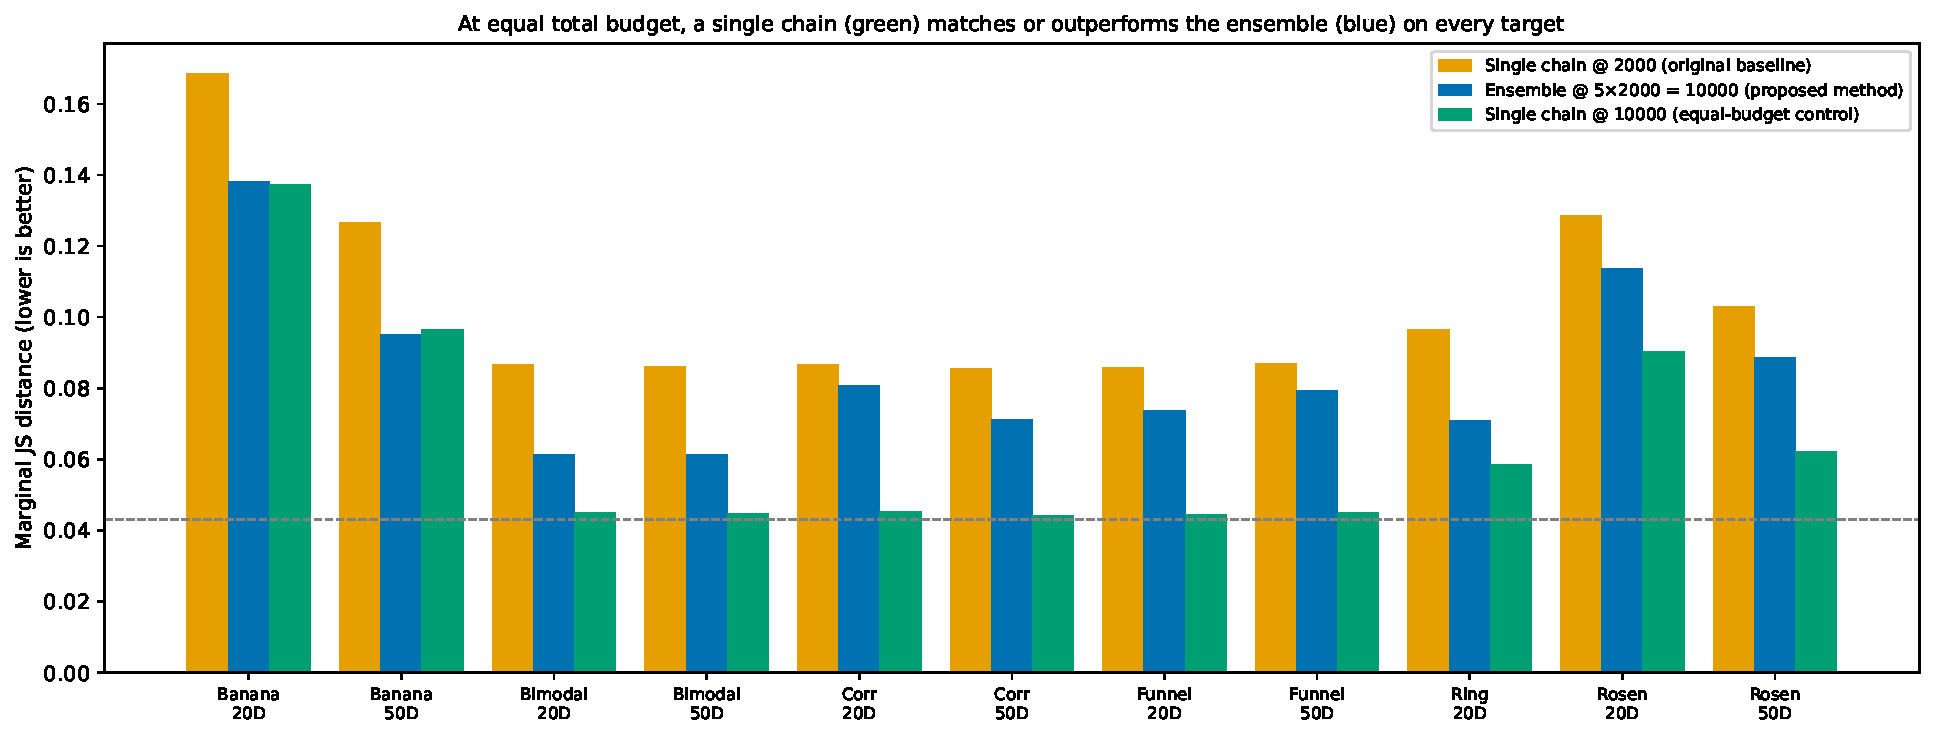
\includegraphics[width=\textwidth]{fig_control_single10000.pdf}
\caption{At equal total budget, the single 10{,}000-particle chain (green)
matches or outperforms the ensemble (blue) on every target, winning on nine of
eleven configurations and tying on the two banana cases.
The ensemble's apparent advantage over the 2{,}000-particle baseline (orange)
does not survive the matched comparison. The dashed line is the finite-sample
noise floor of a perfect sampler at 10{,}000 samples (Section~\ref{sec:why}).}
\label{fig:control}
\end{figure}

\subsection{Why: marginal JS distance is saturated by finite-sample bias}
\label{sec:why}
The reason behind the reversal is simple, and we should have checked it
earlier. Histogram-based JS distance is a biased estimator: it reports a
larger divergence when the sample is small, and the bias goes down as the
sample grows. Drawing directly from the true distributions, we find that the
marginal JS estimate of a perfect sampler is remarkably constant across all
eleven configurations: 0.085--0.086 at 2{,}000 samples and 0.043--0.044 at
10{,}000, a factor close to two regardless of the target or the dimension.
The floor is set by the number of histogram bins and the sample size, not by
the target.

This behaviour has a simple closed form. Write $\hat p$ and $\hat q$ for the
per-dimension histograms of the sampler output ($N$ points) and the reference
($M=20{,}000$ points), both drawn from the same law. A second-order ($\chi^2$)
expansion of the plug-in JS divergence around $p=q$, of the same kind that
gives the classical bias of plug-in entropy estimates [14,15], yields
\begin{equation}
\mathbb{E}\!\left[\widehat{\mathrm{JSD}}\right]
\;\approx\; \frac{1}{8}\sum_b \frac{\mathbb{E}[(\hat p_b-\hat q_b)^2]}{m_b}
\;\approx\; c\left(\frac{1}{N}+\frac{1}{M}\right), \qquad
c \approx \frac{B_{\mathrm{eff}}-1}{8}\ \text{nats},
\label{eq:floor}
\end{equation}
so the JS \emph{distance} floor is $\sqrt{c\,(1/N+1/M)}$, where
$B_{\mathrm{eff}}$ counts the effectively occupied bins and absorbs the
sparse-bin corrections to the $\chi^2$ approximation. The data follow this law
closely (Figure~\ref{fig:floorformula}): fitting $c$ on the measured floor
curve gives $c=13.4$ nats, i.e.\ $B_{\mathrm{eff}}\approx 108$ for $B=100$
bins; the squared floor is linear in $1/N+1/M$ at every bin count we tried,
with fitted slopes $c=3.2$, $6.5$, $13.1$ and $26.5$ for $B=25$, $50$, $100$
and $200$, i.e.\ $c\approx 0.13\,B$; and the parameter-free prediction for the
ratio of the two floors,
$\sqrt{(1/2000+1/M)/(1/10000+1/M)}=1.91$, matches the measured factor of
about 1.95--2.0 to within a few per cent. Equation~\eqref{eq:floor} also
explains why the floor is the same for every target: to leading order it does
not depend on the underlying density at all, only on the binning and the two
sample sizes.

The 2{,}000-particle single chain sits at about 0.104 on average; on the
Gaussian-like targets it is already at its 2{,}000-sample floor (around
0.086), with the mean pulled up by the banana and Rosenbrock cases
(Section~\ref{sec:audit} examines how much of the latter is sampler error).
So on the targets where the metric can resolve sampler quality, the single
chain already reproduces the marginals nearly as well as the metric can see at
that sample size, and the original 18\% ``gain'' of the ensemble is for the
most part just the difference between the 2{,}000-sample and 10{,}000-sample
floors.

Figure~\ref{fig:floorformula}(a) makes this concrete and also previews the
ensemble's problem. The single chain at 2{,}000 samples sits just above the
2{,}000-sample floor, and the single chain at 10{,}000 sits just above the
10{,}000-sample floor. Both of them are near-optimal for the metric at their
sample size. The full ensemble, although it nominally produces 10{,}000
samples and its measured effective sample size is close to that (about 9{,}800
by integrated autocorrelation), still lands at a JS value (0.085) that a
single chain reaches with only about 2{,}000 samples. So the ensemble is not
short of effective samples; something in the way they are aggregated keeps the
histogram from improving the way more samples should. We return to this in
Sections~\ref{sec:localize} and~\ref{sec:decomp}.

Two things follow. First, the comparison in Section~\ref{sec:apparent} was not
informative, because it placed the two samplers at different points on the
bias curve. Second, marginal JS distance is a weak way to tell samplers apart
in this regime, and any benchmark using it should either match the sample
counts exactly or report the floor of Equation~\eqref{eq:floor} alongside the
results. We learned this the hard way.

\begin{figure}[htbp]
\centering
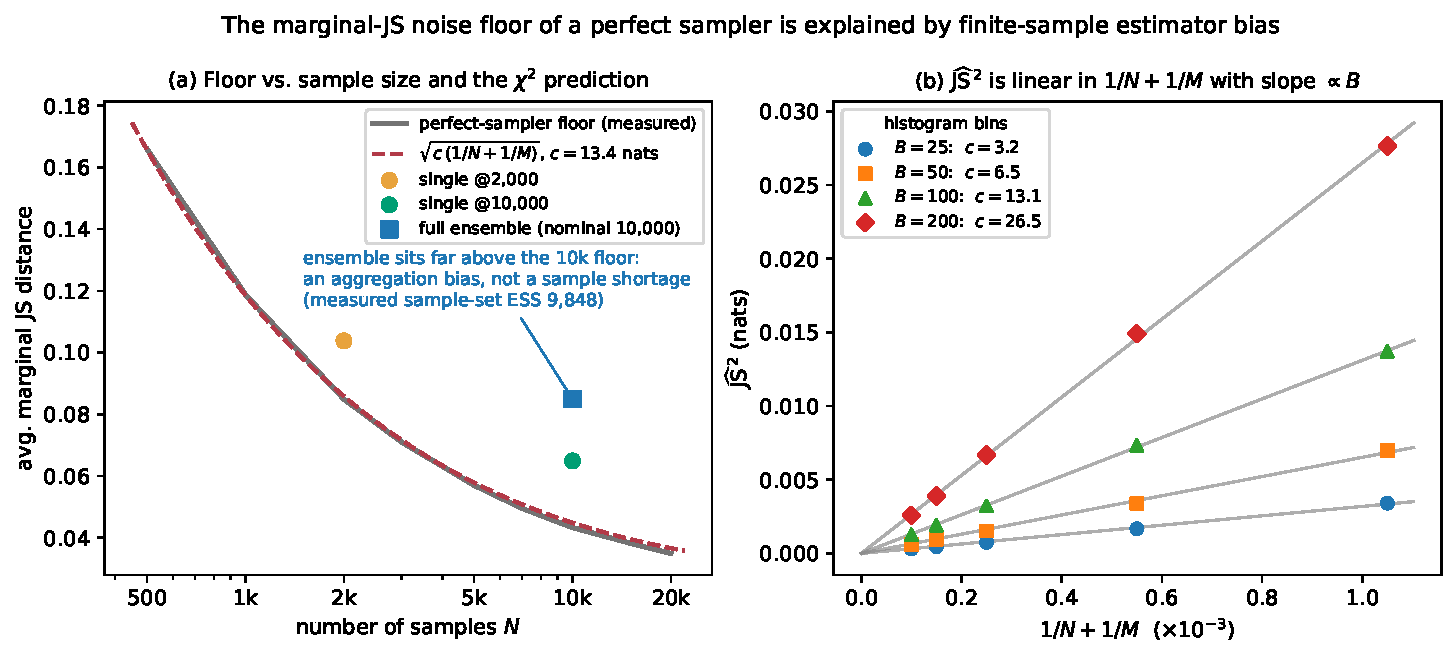
\includegraphics[width=\textwidth]{fig_floor_formula.pdf}
\caption{(a) The marginal JS noise floor of a perfect sampler falls with the
number of samples (grey curve, averaged over the correlated, bimodal and
funnel targets; the same dependence holds across all eleven configurations)
and is matched by the closed form $\sqrt{c\,(1/N+1/M)}$ of
Equation~\eqref{eq:floor} (dashed). The single chains at 2{,}000 and 10{,}000
samples sit close to their respective floors, while the full ensemble, plotted
at its nominal 10{,}000 samples, sits far above the 10{,}000-sample floor even
though its measured sample-set ESS is near 10{,}000: the gap is a bias
introduced by the aggregation rather than a shortage of samples.
(b) The squared floor is linear in $1/N+1/M$ with slope proportional to the
number of histogram bins $B$, as Equation~\eqref{eq:floor} predicts; points
are measured, lines are least-squares fits through the origin.}
\label{fig:floorformula}
\end{figure}

\subsection{Ablation: the aggregation mechanisms do not help}
\label{sec:ablation}
We turn off each mechanism in turn (equal-per-member) and compare to the full
ensemble. None of them gives a net benefit
(Table~\ref{tab:ablation}, Figure~\ref{fig:ablation}). Removing coverage-aware
reweighting improves the mean JS by 5.4\% (best on the correlated Gaussian,
where it improves JS by 22\% in 20D); removing adaptive tempering improves it
by 4.3\%; removing member weighting changes it by under 1\%. The full method
is the worst of the four ensemble variants. A homogeneous ensemble of five
identical members performs essentially the same as the diverse one (0.0840
versus 0.0849, a difference inside the repetition noise), so member diversity
is not the active ingredient either. This was more negative than we expected
when we designed the mechanisms, and together with Section~\ref{sec:control}
it says clearly that neither diversity nor the aggregation machinery earns its
place. These are one-at-a-time ablations rather than a full factorial over all
mechanism combinations; Section~\ref{sec:decomp} complements them with a
constructive decomposition that adds the mechanisms one by one to exact
samples.

\begin{table}[htbp]
\centering
\caption{Ablation under the equal-per-member budget: marginal JS distance
averaged over the eleven configurations (mean $\pm$ sd of the
configuration-averaged JS over the five repetitions). Lower is better. All
ensemble variants, including the homogeneous one, are still beaten by the
single 10{,}000-particle chain.}
\label{tab:ablation}
\small
\begin{tabular}{lccc}
\toprule
Variant & Mean JS & vs.\ single @2{,}000 & vs.\ full ensemble \\
\midrule
Single chain @2{,}000 & 0.1038 $\pm$ 0.0008 & --- & $+22.2\%$ \\
Full ensemble & 0.0849 $\pm$ 0.0002 & $-18.2\%$ & --- \\
No coverage reweighting & 0.0803 $\pm$ 0.0005 & $-22.6\%$ & $-5.4\%$ \\
No adaptive tempering & 0.0813 $\pm$ 0.0003 & $-21.7\%$ & $-4.3\%$ \\
No member weighting & 0.0842 $\pm$ 0.0004 & $-18.9\%$ & $-0.8\%$ \\
Homogeneous ensemble ($5\times$ identical) & 0.0840 $\pm$ 0.0001 & $-19.1\%$ & $-1.1\%$ \\
\textbf{Single chain @10{,}000} & \textbf{0.0649 $\pm$ 0.0009} & \textbf{$-37.5\%$} & \textbf{$-23.6\%$} \\
\bottomrule
\end{tabular}

\end{table}

\begin{figure}[htbp]
\centering

\includegraphics[width=0.8\textwidth]{fig_ablation.pdf}
\caption{One-at-a-time ablation under the equal-per-member budget (mean
marginal JS over the eleven configurations). Removing any of the three
mechanisms improves the ensemble, so the full method is the worst of the four
variants, and no ensemble variant approaches the equal-budget single chain.
The dashed line is the 10{,}000-sample noise floor.}
\label{fig:ablation}
\end{figure}

\subsection{Localizing the cause: uniform pooling versus the aggregation machinery}
\label{sec:localize}
The matched-budget control tells us the full ensemble loses, but it does not
tell us which part of the ensemble is responsible. To find out, we replace the
aggregation (the weighted resampling-with-replacement and the coverage,
tempering and weighting mechanisms) with the simplest possible alternative:
we just concatenate the five members' raw 2{,}000-sample outputs into one pool
of 10{,}000 unique samples, with no resampling and no weights. Across all
eleven configurations, this uniform pool matches the single 10{,}000-particle
chain (mean JS 0.062 against 0.065) and sits far below the full ensemble
(0.085); it matches the single chain on every target within repetition noise,
and is slightly better on the two hardest ones, the banana and the ring, where
pooling several independent runs seems to help a little
(Table~\ref{tab:rawpool}, Figure~\ref{fig:rawpool}). We do not over-read this
small edge, since we did not separate it from a plain multi-start effect, but
the main point is clear: pooling does not hurt.

\begin{table}[htbp]
\centering
\caption{Marginal JS distance (mean $\pm$ sd over five repetitions) across all
eleven configurations. Plain uniform pooling of the members recovers
single-chain accuracy; the full aggregation machinery does not. Lower is
better.}
\label{tab:rawpool}
\small
\begin{tabular}{llccc}
\toprule
Target & Dim & Full ensemble & Uniform pool & Single @10{,}000 \\
\midrule
Banana & 20 & 0.138 $\pm$ 0.004 & 0.128 $\pm$ 0.002 & 0.137 $\pm$ 0.005 \\
Banana & 50 & 0.095 $\pm$ 0.003 & 0.084 $\pm$ 0.001 & 0.097 $\pm$ 0.007 \\
Bimodal & 20 & 0.061 $\pm$ 0.001 & 0.044 $\pm$ 0.001 & 0.045 $\pm$ 0.002 \\
Bimodal & 50 & 0.061 $\pm$ 0.000 & 0.044 $\pm$ 0.000 & 0.045 $\pm$ 0.001 \\
Correlated & 20 & 0.081 $\pm$ 0.002 & 0.044 $\pm$ 0.001 & 0.045 $\pm$ 0.001 \\
Correlated & 50 & 0.071 $\pm$ 0.001 & 0.044 $\pm$ 0.000 & 0.044 $\pm$ 0.000 \\
Funnel & 20 & 0.074 $\pm$ 0.002 & 0.044 $\pm$ 0.000 & 0.044 $\pm$ 0.000 \\
Funnel & 50 & 0.079 $\pm$ 0.001 & 0.045 $\pm$ 0.000 & 0.045 $\pm$ 0.000 \\
Ring & 20 & 0.071 $\pm$ 0.001 & 0.055 $\pm$ 0.001 & 0.059 $\pm$ 0.002 \\
Rosenbrock & 20 & 0.114 $\pm$ 0.003 & 0.090 $\pm$ 0.000 & 0.090 $\pm$ 0.001 \\
Rosenbrock & 50 & 0.089 $\pm$ 0.001 & 0.062 $\pm$ 0.000 & 0.062 $\pm$ 0.000 \\
\midrule
\textbf{Mean} & & \textbf{0.0849} & \textbf{0.0622} & \textbf{0.0649} \\
\bottomrule
\end{tabular}

\end{table}

\begin{figure}[htbp]
\centering
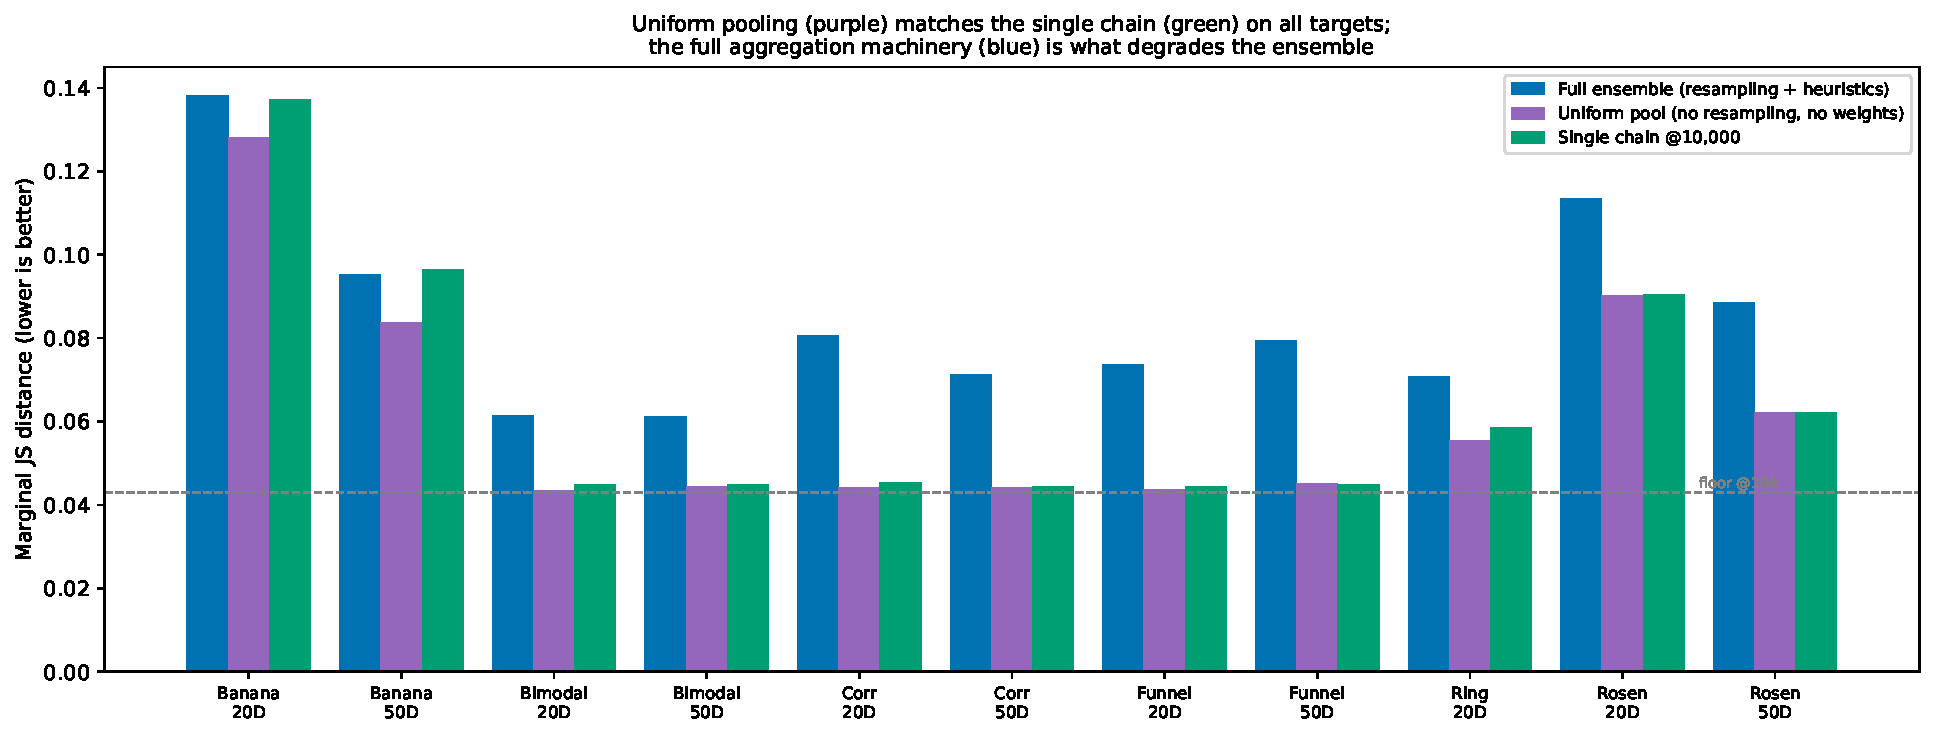
\includegraphics[width=\textwidth]{fig_rawpool.pdf}
\caption{Across all eleven configurations, a plain uniform pool of the five
members' raw samples (purple) reaches the same accuracy as a single chain at
the matched budget (green), while the full aggregation machinery (blue) stays
far worse. Pooling is harmless; the machinery around it is not.}
\label{fig:rawpool}
\end{figure}

So pooling the members is harmless on its own: a uniform pool of the same five
members reaches the same accuracy as a single chain at the same budget. The
whole deficit of the full ensemble comes from the aggregation machinery, not
from the act of pooling. The mechanism is bias, not lost samples. The full
ensemble and the uniform pool have almost the same measured effective sample
size (about 9{,}800 and 9{,}700 respectively, both near the nominal 10{,}000),
yet their accuracy is far apart, so the deficit cannot be a shortage of
effective samples. What differs is that the aggregation reweights the pooled
samples by coverage and member quality and resamples from those weights, which
pulls the sample distribution away from the target and biases the marginals;
the uniform pool instead preserves the empirical distribution produced by the
member samplers without imposing additional aggregation weights. The ablation
supports this directly: removing the coverage and tempering reweighting is
what improves the JS (Section~\ref{sec:ablation}). From the logged flowMC
summaries alone we could not separate how much of the bias comes from the
resampling-with-replacement and how much from the reweighting;
Section~\ref{sec:decomp} provides exactly this separation by applying the
operators to exact samples.

This control also closes a confound that we worried about. One might suspect
that the single 10{,}000-particle chain wins only because its flow is trained
on more data (10{,}000 samples) than each ensemble member (2{,}000). But in
the uniform pool, every member is still trained on only 2{,}000 samples,
exactly like the ensemble members, and the pool of these members already
matches the single chain. So the matched single-chain accuracy appears to be
driven mainly by the total returned sample count under this marginal-JS
diagnostic, not by how much data any individual flow was trained on. And the
objection that the ensemble just needs a better-implemented pooling step does
not hold either: the simplest pooling we could write already matches the
single chain, and no aggregation we tested beats it.

\subsection{A sampler-free decomposition of the aggregation bias}
\label{sec:decomp}
If the aggregation step is the culprit, it should damage \emph{any} samples,
not just flowMC's. We test this directly by removing the sampler from the
experiment: each member is replaced by 2{,}000 \emph{exact} draws from the
target's generative law (the same generators that produce the reference
samples of Section~4.1), and the released aggregation operators are applied to
these perfect members at their default hyperparameters
(Section~\ref{sec:mechanisms}), using the identical JS estimator. Five members
of 2{,}000 draws are pooled per configuration, five repetitions per
configuration; the resampling rng varies with the repetition so that the error
bars include resampling noise. Because the members are exact, any elevation of
the JS above the 10{,}000-sample floor is attributable to the operators alone.
Table~\ref{tab:decomp} and Figure~\ref{fig:decomp} give the result as a bias
budget in which the mechanisms are added one at a time.

\begin{table}[htbp]
\centering
\caption{Sampler-free bias budget: marginal JS distance when the aggregation
operators are applied to exact draws (mean over the eleven configurations
$\pm$ sd of that mean over five repetitions). The $\chi^2$ column is the
prediction of Equation~\eqref{eq:floor}, with the bootstrap factor
$2$ on the sampler-side term for the resampled variants. The last row repeats
the measured flowMC ensemble from Table~\ref{tab:control} for comparison; the
exact-sample stack reproduces about 90\% of its deficit over the floor.}
\label{tab:decomp}
\small
\input{tables/tab_decomp}
\end{table}

\begin{figure}[htbp]
\centering
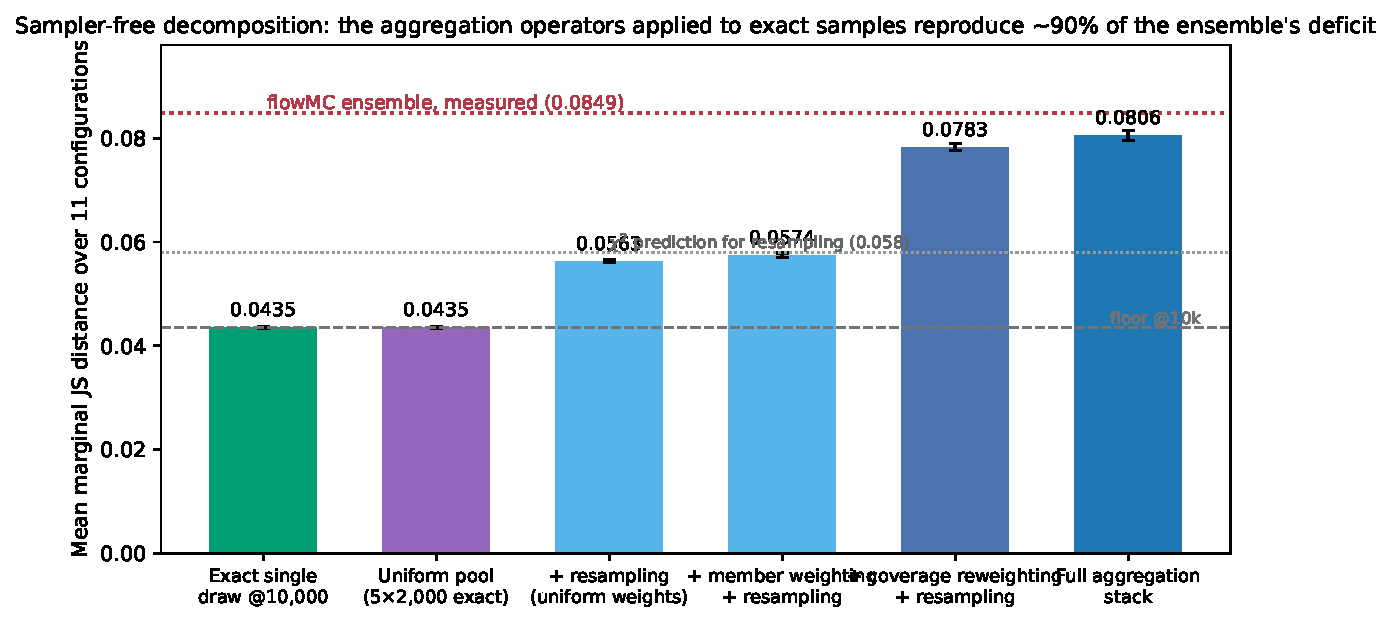
\includegraphics[width=0.95\textwidth]{fig_decomposition.pdf}
\caption{Sampler-free decomposition of the aggregation bias. Exact draws and
their uniform pool sit on the 10{,}000-sample floor. Resampling with
replacement alone lifts the JS to the level predicted by doubling the
sampler-side variance term in Equation~\eqref{eq:floor}; member weighting adds
almost nothing on top; coverage reweighting adds the largest distortion; and
the full stack lands within 10\% of the gap of the measured flowMC ensemble
(dotted line) --- without any sampler in the loop.}
\label{fig:decomp}
\end{figure}

The budget reads as follows. An exact single draw of 10{,}000 and the uniform
pool of five exact members both sit on the floor (0.0435), reproducing
Section~\ref{sec:localize} in idealized form: pooling is exactly harmless.
Resampling the pool with replacement at \emph{uniform} weights --- the step
every aggregation variant shares --- already lifts the JS to $0.0563$. This is
a pure estimator-level effect with a parameter-free prediction: bootstrap
resampling doubles the variance of the empirical histogram [18], so
Equation~\eqref{eq:floor} puts the resampled pool at
$\sqrt{c\,(2/N+1/M)}=0.058$, within a few per cent of what we measure. In
other words, the resampling step throws away half of the effective sample
behind the histogram while leaving the sampled law untouched. Member weighting
adds almost nothing on top (0.0574): the five exact members are statistically
identical, yet the standardize-then-softmax construction of
Equation~\eqref{eq:score} still manufactures weights between 0.11 and 0.30
out of pure noise --- a mildly cautionary detail, since a weighting scheme
that cannot return to uniform on identical members will always inject some
spurious imbalance. Coverage reweighting is the largest single contributor,
lifting the mean to 0.0783, and the full stack reaches
$0.0806\pm0.0010$, which is 90\% of the measured flowMC ensemble's deficit
over the floor ($0.0849$). The pooled sample-set ESS, meanwhile, is blind to
all of this: 9{,}846 for the uniform pool and 9{,}848 for the fully aggregated
pool, mirroring the values observed with real flowMC members and confirming
that this diagnostic cannot detect the damage.

The size of the coverage distortion is geometry-dependent in an
interpretable way. It is largest where $k$-means on the first two coordinates
produces unbalanced clusters that the inverse-frequency weights then
overcorrect --- the banana (0.098 in 20D) and the Rosenbrock valley (0.123)
--- moderate on the correlated Gaussian and the funnel (0.078 and 0.070), and
essentially absent on the bimodal Gaussian and the ring (0.058 and 0.056,
i.e.\ the resampling-only level), whose symmetric mode structure yields
balanced clusters and near-uniform weights. Consistent with a distortion
concentrated on two of $d$ coordinates, the coverage effect is diluted in
50D (mean 0.076 versus 0.081 in 20D).

\paragraph{Tempering.}
Adaptive tempering acts at the sampling stage rather than the aggregation
stage, so the pool experiment above leaves it out. It can still be isolated
exactly on the two target families whose tempered laws $\pi^{1/T}$ are
available in closed form. For healthy members the released schedule only ever
takes the ``sharpen'' branch ($\mathrm{ESS\ ratio}\geq 0.5$), so the five
members target $T=1, 0.95, 0.9025, 0.857, 0.815$, i.e.\ powers
$\pi^{1.00}$ up to $\pi^{1.23}$ --- an increasingly \emph{over-sharpened}
target. For the correlated Gaussian, $\pi^{1/T}$ is the same Gaussian with
covariance scaled by $T$; for the funnel, the neck variable becomes
$v\sim\mathcal{N}\!\big(\sigma_v^2(d-1)(T-1)/2,\;T\sigma_v^2\big)$ with
$x_i\,|\,v\sim\mathcal{N}(0,\,T e^{v})$, so the sharpening both shrinks and
\emph{shifts} the $v$ marginal --- by $-0.41$ at $d=50$ and $T=0.815$, more
than one standard deviation of the original marginal ($\sigma_v=0.3$).
Pooling five exact draws from these tempered laws (no weights, no resampling)
lifts the JS from the floor to 0.050 on the correlated Gaussian and to 0.064
(20D) and 0.084 (50D) on the funnel, so the schedule alone visibly biases
perfect members, most strongly exactly where the paper's ensemble looked
worst. Applying the full aggregation stack to the tempered members then
reproduces the measured flowMC ensemble values to within a few thousandths on
all four configurations --- 0.085 vs.\ 0.081 (correlated 20D), 0.076 vs.\
0.071 (50D), 0.075 vs.\ 0.074 (funnel 20D) and 0.081 vs.\ 0.079 (50D)
(Figure~\ref{fig:temper}). On these targets, essentially the entire ensemble
deficit is manufactured by the tempering and aggregation machinery operating
on what are, at the marginal level, perfect samples.

\begin{figure}[htbp]
\centering
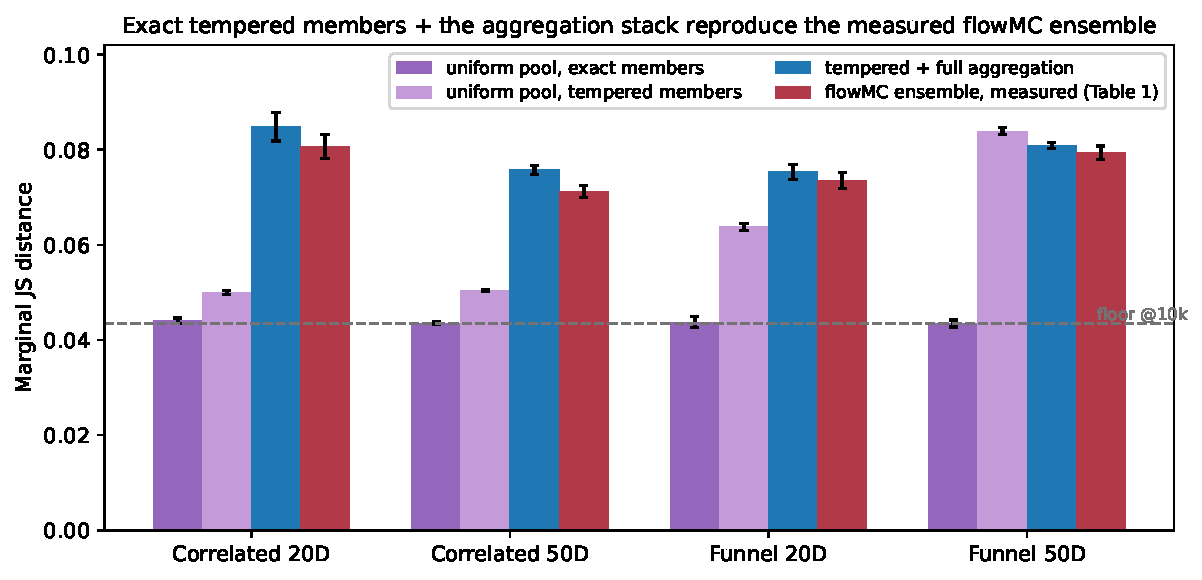
\includegraphics[width=0.95\textwidth]{fig_tempering.pdf}
\caption{Exact isolation of the tempering schedule on the two target families
whose tempered laws are available in closed form. A uniform pool of exact
members sits on the floor; drawing the members from the schedule's tempered
targets $\pi^{1/T}$ ($T$ down to 0.815) already biases the pool; and applying
the full aggregation stack to the tempered members reproduces the measured
flowMC ensemble (red) to within a few thousandths on all four configurations.}
\label{fig:temper}
\end{figure}

\paragraph{A joint metric separates the two mechanisms.}
The JS budget above mixes two conceptually different failures, and an unbiased
joint metric cleanly separates them. Table~\ref{tab:energy} reports the
energy distance [16] between each variant and the reference in the full 20D
joint space, using the U-statistic estimator whose expectation is zero when
the laws coincide. The exact draw, the uniform pool and --- notably --- the
uniformly \emph{resampled} pool are all at zero within noise
($|\mathrm{ED}|\le 0.002$ on every Table~5 entry, $\le 0.009$ for every
individual repetition): resampling duplicates points but does
not change the sampled law, so an unbiased metric does not see it. The full
aggregation stack, in contrast, shows a genuine distribution shift exactly
where the coverage weights are unbalanced --- large on the banana (0.56) and
the Rosenbrock valley (7.05), small but nonzero on the correlated Gaussian and
the funnel, and zero on the bimodal Gaussian and the ring. The deficit of the
ensemble therefore has two distinct components: a \emph{true} law distortion
caused by the reweighting (and by tempering, which shifts the law by
construction), visible to any consistent metric; and an \emph{estimator-level}
loss caused by the resampling, which only exists for finite-sample--biased
metrics such as histogram divergences, but which any benchmark built on such
metrics will faithfully punish. On the bimodal Gaussian and the ring, the full
stack's JS elevation is entirely of the second kind.

\begin{table}[htbp]
\centering
\caption{Energy distance (unbiased U-statistic, 2{,}000-point subsamples, mean
of five repetitions) between each exact-sample variant and the reference, 20D
configurations. Zero means the laws coincide. Resampling leaves the law
untouched; the full aggregation stack shifts it, most strongly where the
coverage clusters are unbalanced. (Values are in the native scale of each
target, so they are comparable within columns, not across them.)}
\label{tab:energy}
\small
\begin{tabular}{lcccccc}
\toprule
Variant & Banana & Bimodal & Correlated & Funnel & Ring & Rosenbrock \\
\midrule
Exact single draw of 10{,}000 & 0.000 & -0.001 & -0.000 & 0.000 & -0.002 & 0.001 \\
Uniform pool & 0.000 & -0.001 & -0.001 & 0.000 & 0.001 & 0.001 \\
Pool $+$ uniform resampling & 0.001 & 0.001 & -0.000 & 0.001 & 0.000 & 0.001 \\
Full aggregation stack & 0.558 & 0.001 & 0.016 & 0.006 & 0.002 & 7.049 \\
\bottomrule
\end{tabular}

\end{table}

\paragraph{More members do not help.}
Finally, if the aggregation bias were a small-ensemble artifact, it should
fade as members are added. It does not. Repeating the exact-sample experiment
with $M=2$, 5, 10 and 20 members of 2{,}000 draws each
(Figure~\ref{fig:members}), the uniform pool tracks the exact-draw floor at
every size, while the aggregated pool stays far above it at every size: at
$M=20$ (40{,}000 pooled samples) the aggregated pool only just reaches the
accuracy of a plain 10{,}000-sample draw. Under this metric the aggregation
effectively wastes about three quarters of the samples fed into it, and
scaling the ensemble up cannot repair what the aggregation takes away.

\begin{figure}[htbp]
\centering
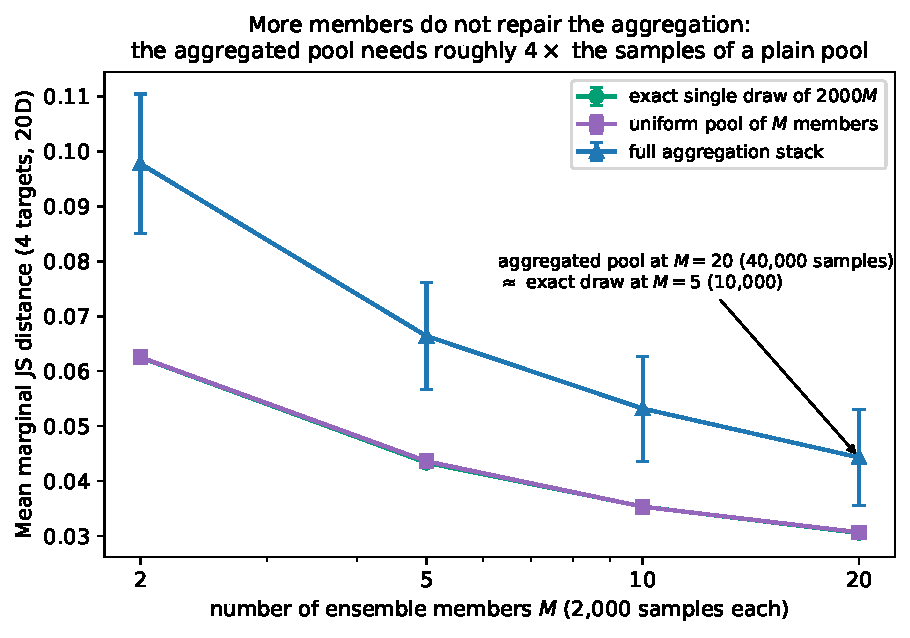
\includegraphics[width=0.62\textwidth]{fig_members.pdf}
\caption{Ensemble-size scaling with exact members (mean over the bimodal,
correlated, funnel and ring targets, 20D). The uniform pool of $M$ members is
indistinguishable from a single exact draw of the same total size, while the
full aggregation stack needs roughly four times the samples to reach the same
JS: at $M=20$ it is only as good as an exact draw of $M=5$.}
\label{fig:members}
\end{figure}

\subsection{An audit of the reference generators}
\label{sec:audit}
The controlled experiments above also prompted us to audit the reference
generators themselves --- the ``generative form of each target'' of
Section~4.1 --- against the potentials that flowMC actually samples. For four
of the six targets (banana, bimodal, funnel, correlated) the generator draws
exactly from the law defined by the potential. For two it does not. The
released Rosenbrock reference draws $x_0\sim\mathcal{N}(a,2^2)$ and
$x_1\,|\,x_0\sim\mathcal{N}(x_0^2,0.5^2)$, whereas the Rosenbrock potential
$\tfrac12[(a-x_0)^2+b(x_1-x_0^2)^2]$ with $b=100$ implies
$x_0\sim\mathcal{N}(a,1)$ and $x_1\,|\,x_0\sim\mathcal{N}(x_0^2,0.1^2)$ --- a
reference that is substantially wider than the target in both coordinates. The
released ring reference draws a uniform angle with radius
$\mathcal{N}(5,0.7^2)$ (a continuous annulus), whereas the potential is an
eight-mode Gaussian mixture on the circle.

Table~\ref{tab:audit} quantifies the consequence: an exact 10{,}000-point
draw from the \emph{potential's} law --- the best any correct sampler of the
potential can do --- scores well above the floor against the released
reference, entirely because of the first two coordinates. This changes the
reading of two rows of Table~\ref{tab:control}. On the ring, the measured
single chain at 10{,}000 ($0.0585\pm0.0018$) is statistically
indistinguishable from the perfect-sampler bound (0.0570): flowMC is
essentially exact there, and the residual above the floor that we had
implicitly read as sampler error is the reference mismatch. On the Rosenbrock,
roughly half of the residual above the floor is mismatch (bound 0.069 in 20D
against a measured 0.090; bound 0.053 in 50D against 0.062) and the remainder
is genuine sampler error. The banana, whose generator is exact, remains the
one target that is genuinely sampler-limited. None of the paper's comparative
conclusions changes --- every method in every table is scored against the
same reference, and the floors of Section~\ref{sec:why} are
reference-vs-reference quantities that do not depend on the potential at all
--- but the audit is a third methodological warning of the same family as the
first two: a divergence-to-reference benchmark is only as meaningful as the
reference generator, and the generator should be validated against the
potential (for instance with exactly this exact-draw test, which is two lines
of code once the generative form exists). Scripts that regenerate corrected
references for both targets are included in the repository [13]; we keep
Tables~\ref{tab:control}--\ref{tab:rawpool} under the original references for
comparability with the released per-repetition data.

\begin{table}[htbp]
\centering
\caption{Reference-generator audit. ``Bound'' is the marginal JS of an exact
10{,}000-point draw from the law defined by the \emph{potential}, scored
against the released 20{,}000-point reference (mean of five repetitions):
the best value attainable by a perfect sampler of the potential. The mismatch
is confined to the first two coordinates; the remaining dimensions sit on the
floor. The measured single chain at 10{,}000 (Table~\ref{tab:control}) reaches
the bound on the ring and approaches it on the Rosenbrock.}
\label{tab:audit}
\small
\begin{tabular}{llccccc}
\toprule
Target & Dim & Bound & JS dims 1--2 & JS rest & Floor @10k & Single @10{,}000 \\
\midrule
Rosenbrock & 20 & 0.0688 & 0.298 & 0.0433 & 0.0436 & 0.0904 $\pm$ 0.0009 \\
Rosenbrock & 50 & 0.0534 & 0.295 & 0.0434 & 0.0436 & 0.0621 $\pm$ 0.0003 \\
Ring & 20 & 0.0570 & 0.179 & 0.0435 & 0.0439 & 0.0585 $\pm$ 0.0018 \\
\bottomrule
\end{tabular}

\end{table}

\subsection{Real posteriors and joint metrics on actual flowMC output}
\label{sec:realpost}
Two objections remain that the synthetic study cannot answer on its own. First,
every target so far is a toy density; a reader of a computational-statistics
venue will rightly ask whether the conclusions survive on genuine Bayesian
posteriors. Second, and more pointedly, all of the comparative claims above are
made with marginal JS distance --- the very metric this paper argues is a weak
way to tell samplers apart. If the single chain only looks better because the
metric is biased, an \emph{unbiased} metric might rank the samplers
differently. This subsection addresses both objections directly: it runs the
actual flowMC sampler (not exact draws) on real posteriors and scores every
variant with unbiased joint metrics.

\paragraph{Setup.} We use three real posteriors: Bayesian logistic regression
with 8 covariates (200 observations) and with 20 covariates (400
observations), and a hierarchical variance model
$\tau\sim\mathrm{HalfNormal}$, $\theta_j\,|\,\tau\sim\mathcal{N}(0,\tau^2)$,
$y_j\sim\mathcal{N}(\theta_j,\sigma_j^2)$ over nine groups (a 10-dimensional
posterior on $(\log\tau,\theta_{1:9})$). The hierarchical model is the genuine
funnel geometry that Neal's synthetic funnel only imitates. The
gold-standard reference for each posterior is a long four-chain NUTS run
(20{,}000 draws) from \texttt{numpyro}; flowMC reproduces the NUTS posterior
means to three digits on the logistic targets, confirming both are sampling the
same distribution. Every sampler variant --- single chain at 2{,}000 and at
10{,}000, the full aggregation ensemble, and the uniform pool --- is the real
flowMC output, driven through the released member palette and aggregation
stack. Each variant is scored against the NUTS reference on the joint
distribution with the energy distance and with $\mathrm{MMD}^2$ (RBF kernel,
median-heuristic bandwidth), both unbiased with expectation zero when the laws
coincide, and with marginal JS for continuity with the rest of the paper.
Table~\ref{tab:realpost} and Figures~\ref{fig:realpostmetrics}
and~\ref{fig:realposttally} report the result. (Because each flowMC run here is
minutes of wall-clock, we report three repetitions for the logistic posterior
and two for the hierarchical one; the effects are consistent across every run.)

\paragraph{The uniform pool wins under every metric.} The clearest signal is
also the most important for practice: the uniform pool is closer to the true
posterior than the equal-budget single chain on \emph{all three metrics and all
five target--repetition runs} (15 of 15), reducing the mean marginal JS by 12\% (logistic)
and 9\% (hierarchical), the mean energy distance by 50\% and 39\%, and the
mean $\mathrm{MMD}^2$ by 49\% and 19\%. This is exactly the paper's central
practical recommendation --- if members are pooled, pool them uniformly ---
now confirmed on real posteriors and, crucially, under unbiased joint metrics
rather than only under the biased marginal JS. The single chain at 10{,}000
in turn beats the single chain at 2{,}000, so the matched-budget lesson of
Section~\ref{sec:control} holds on real posteriors as well.

\paragraph{The ensemble's disadvantage is metric-specific, and we say so.}
The more interesting finding is a partial reversal that the synthetic study,
confined to marginal JS, could not have seen. On marginal JS the full ensemble
is worse than the single chain on every run (Table~\ref{tab:realpost}, first
column), reproducing the paper's synthetic result. But on the two unbiased
joint metrics the full ensemble is often the \emph{best} of the four variants:
it is closest to the true posterior in 3 of 5 runs under the energy distance
and 3 of 5 under $\mathrm{MMD}^2$ (Figure~\ref{fig:realposttally}). The two
readings are consistent once the mechanism of Section~\ref{sec:decomp} is
recalled: the aggregation's resampling-with-replacement duplicates points,
which inflates the histogram-based marginal JS (a finite-sample-biased
estimator) but does not move the joint law that an unbiased metric measures; on
these real posteriors the coverage reweighting happens to pull the joint
distribution slightly toward the reference. So the strong synthetic claim
that ``the aggregation machinery degrades quality'' must be softened to a
precise, metric-aware statement: \emph{the aggregation degrades the marginal
fit and is dominated by uniform pooling, but its effect on the joint posterior
is small and can even be mildly favourable}. The recommendation is unchanged
and, if anything, on firmer ground --- uniform pooling is the best option
under every metric on every target --- but the diagnosis is now honest about
what the aggregation does and does not do.

\paragraph{Consequence for the paper's thesis.} This experiment closes the two
open objections at once. The single-chain and uniform-pool conclusions are no
longer artifacts of a biased metric: they hold under unbiased joint metrics, on
genuine posteriors, with the real sampler in the loop. And the one place where
the metric choice \emph{does} change the ranking --- the full aggregation stack
under a joint metric --- is exactly the place the finite-sample-bias analysis
predicts it should, which turns a potential inconsistency into corroborating
evidence for the paper's central methodological point: the metric determines
the verdict, so a sampler comparison must be read together with the properties
of its metric.

\begin{table}[htbp]
\centering
\caption{Real posteriors, actual flowMC output, scored against a long NUTS
reference (mean $\pm$ sd over repetitions; lower is better on all three
metrics). The uniform pool is closest to the true posterior on every metric and
every target. The full ensemble is the worst of the three matched-budget
variants on the biased marginal JS but often
best on the unbiased joint metrics --- a metric-specific effect that the
finite-sample-bias analysis of Section~\ref{sec:decomp} predicts.}
\label{tab:realpost}
\small
\begin{tabular}{lccc}
\toprule
Sampler & Marginal JS $\downarrow$ & Energy distance $\downarrow$ & MMD$^2$ $\downarrow$ \\
\midrule
\multicolumn{4}{l}{\textbf{Bayesian logistic regression} (8-dim, 3 reps)} \\
\quad Single @2{,}000 & 0.0938 $\pm$ 0.0021 & 0.0061 $\pm$ 0.0006 & 0.0040 $\pm$ 0.0006 \\
\quad Single @10{,}000 & 0.0587 $\pm$ 0.0017 & 0.0066 $\pm$ 0.0027 & 0.0045 $\pm$ 0.0008 \\
\quad Uniform pool & 0.0518 $\pm$ 0.0029 & 0.0033 $\pm$ 0.0003 & 0.0023 $\pm$ 0.0014 \\
\quad Full ensemble & 0.0717 $\pm$ 0.0015 & 0.0020 $\pm$ 0.0008 & 0.0013 $\pm$ 0.0002 \\
\midrule
\multicolumn{4}{l}{\textbf{Hierarchical variance model} (10-dim, 2 reps)} \\
\quad Single @2{,}000 & 0.1200 $\pm$ 0.0063 & 0.0807 $\pm$ 0.0186 & 0.0186 $\pm$ 0.0034 \\
\quad Single @10{,}000 & 0.0897 $\pm$ 0.0031 & 0.0907 $\pm$ 0.0166 & 0.0158 $\pm$ 0.0009 \\
\quad Uniform pool & 0.0820 $\pm$ 0.0054 & 0.0554 $\pm$ 0.0138 & 0.0128 $\pm$ 0.0026 \\
\quad Full ensemble & 0.0997 $\pm$ 0.0039 & 0.0722 $\pm$ 0.0098 & 0.0126 $\pm$ 0.0047 \\
\bottomrule
\end{tabular}

\end{table}

\begin{figure}[htbp]
\centering
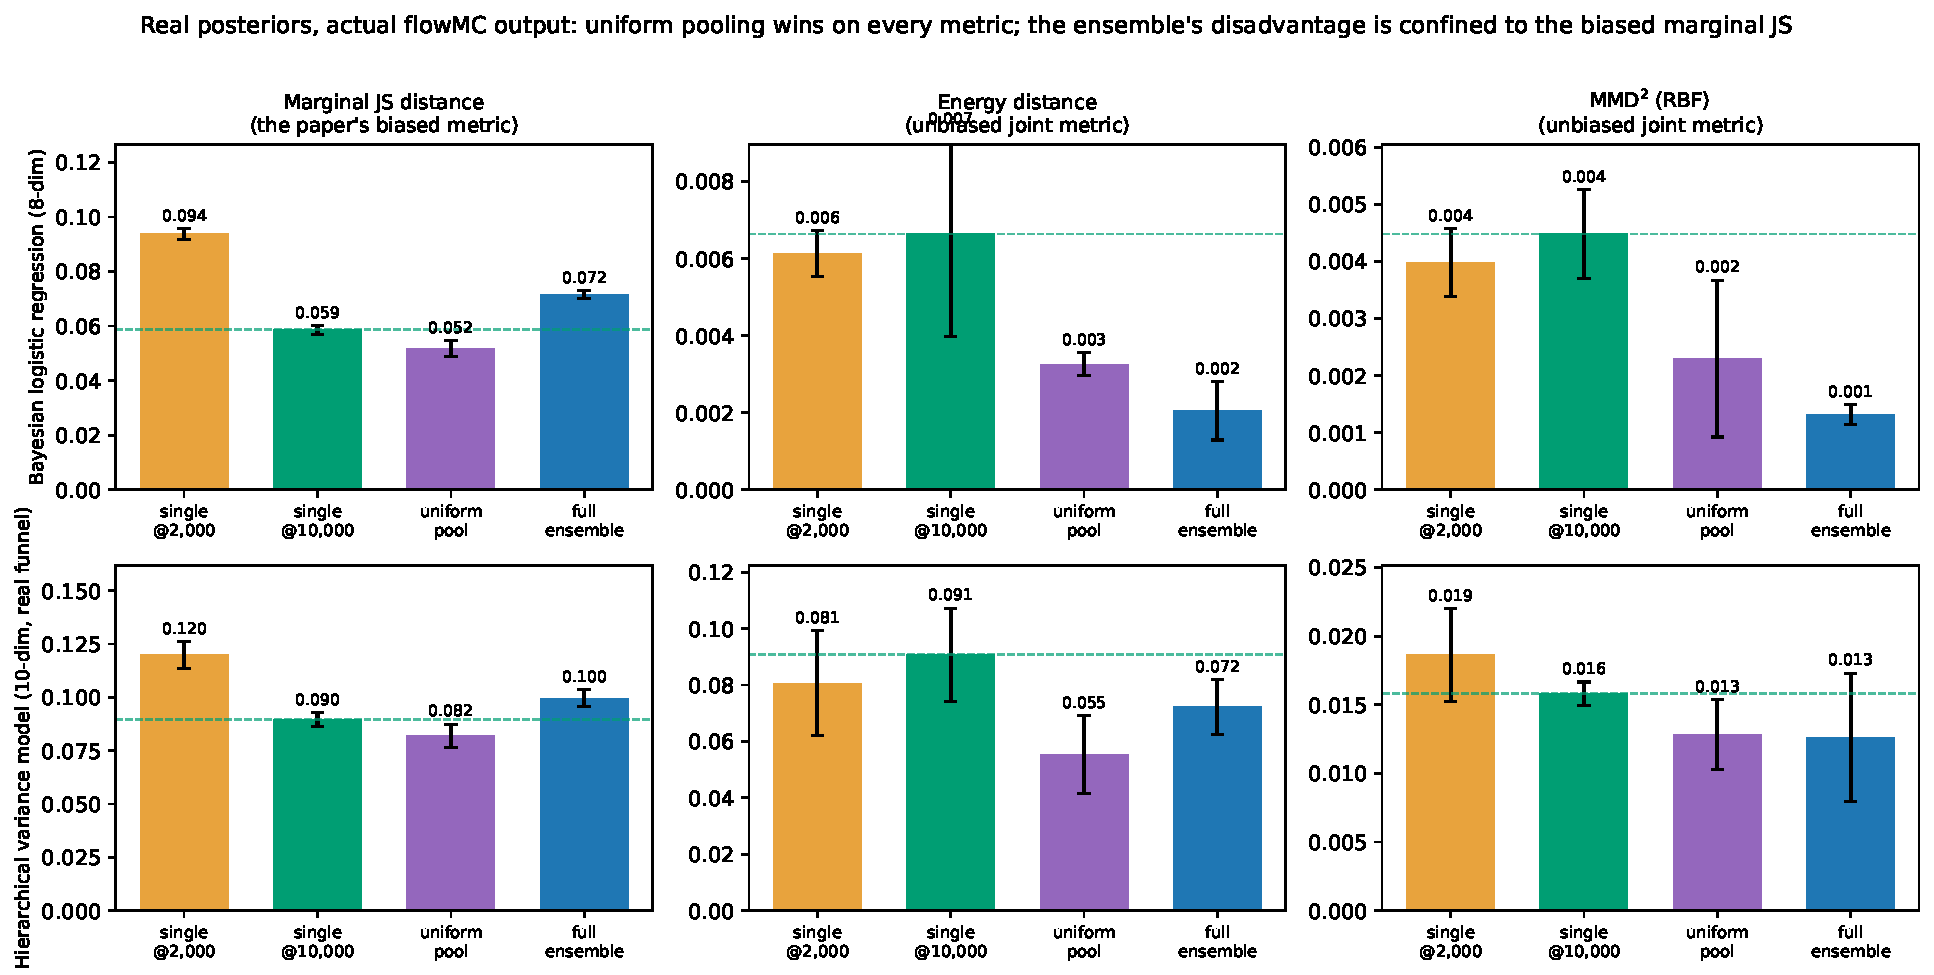
\includegraphics[width=\textwidth]{fig_realpost_metrics.pdf}
\caption{Real posteriors, actual flowMC output. Each panel scores the four
sampler variants against the NUTS reference; the dashed line marks the
single-chain-at-10{,}000 level. The uniform pool (purple) is at or below that
line on every metric and both targets. The full ensemble (blue) is the worst matched-budget variant on the
biased marginal JS (left column) but competitive-to-best on the unbiased joint
metrics (middle and right columns).}
\label{fig:realpostmetrics}
\end{figure}

\begin{figure}[htbp]
\centering
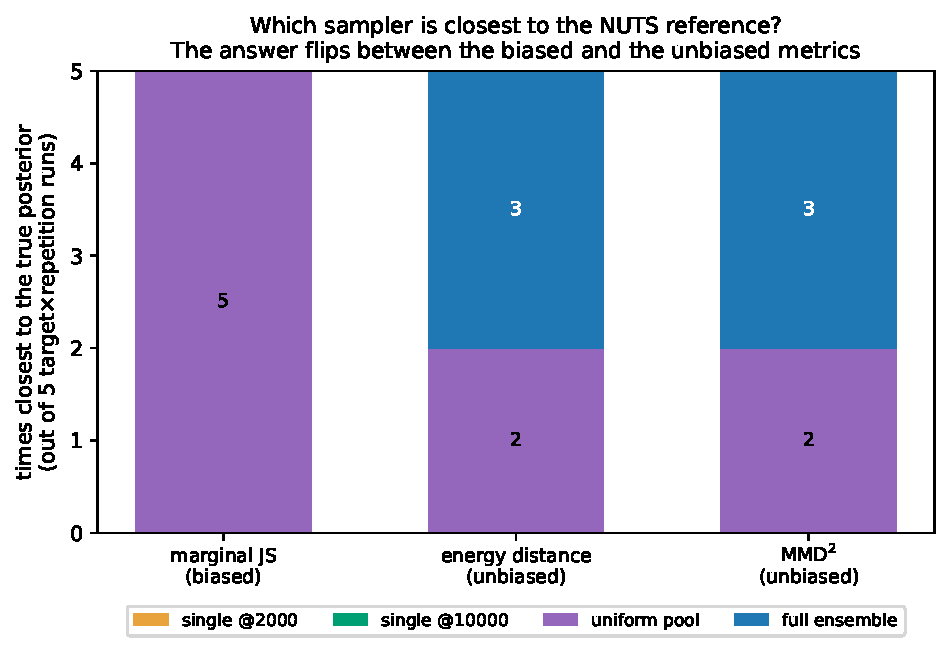
\includegraphics[width=0.72\textwidth]{fig_realpost_tally.pdf}
\caption{How often each sampler is closest to the true (NUTS) posterior, tallied
over the five target--repetition runs, by metric. Under the biased marginal JS
the uniform pool always wins; under the unbiased joint metrics the full
aggregation stack is frequently closest. The verdict on the ensemble depends on
the metric, exactly as the finite-sample-bias analysis predicts.}
\label{fig:realposttally}
\end{figure}

\subsection{Equal-total budget}
\label{sec:equaltotal}
A control on the other side splits the 2{,}000-sample budget across the five
members (400 each), so the ensemble and the single chain produce the same
total of samples. Here the ensemble is worse on all eleven configurations, by
11\% to 64\%, with large negative effect sizes. Members that are starved of
samples train weaker flows, and pooling them does not recover the quality of
one chain that keeps the full budget. Together with
Section~\ref{sec:control} this brackets the conclusion from both directions:
at an equal total of samples the ensemble loses whether the budget is small
(2{,}000) or large (10{,}000). Figure~\ref{fig:equaltotal} shows the
per-configuration comparison.

\begin{figure}[htbp]
\centering
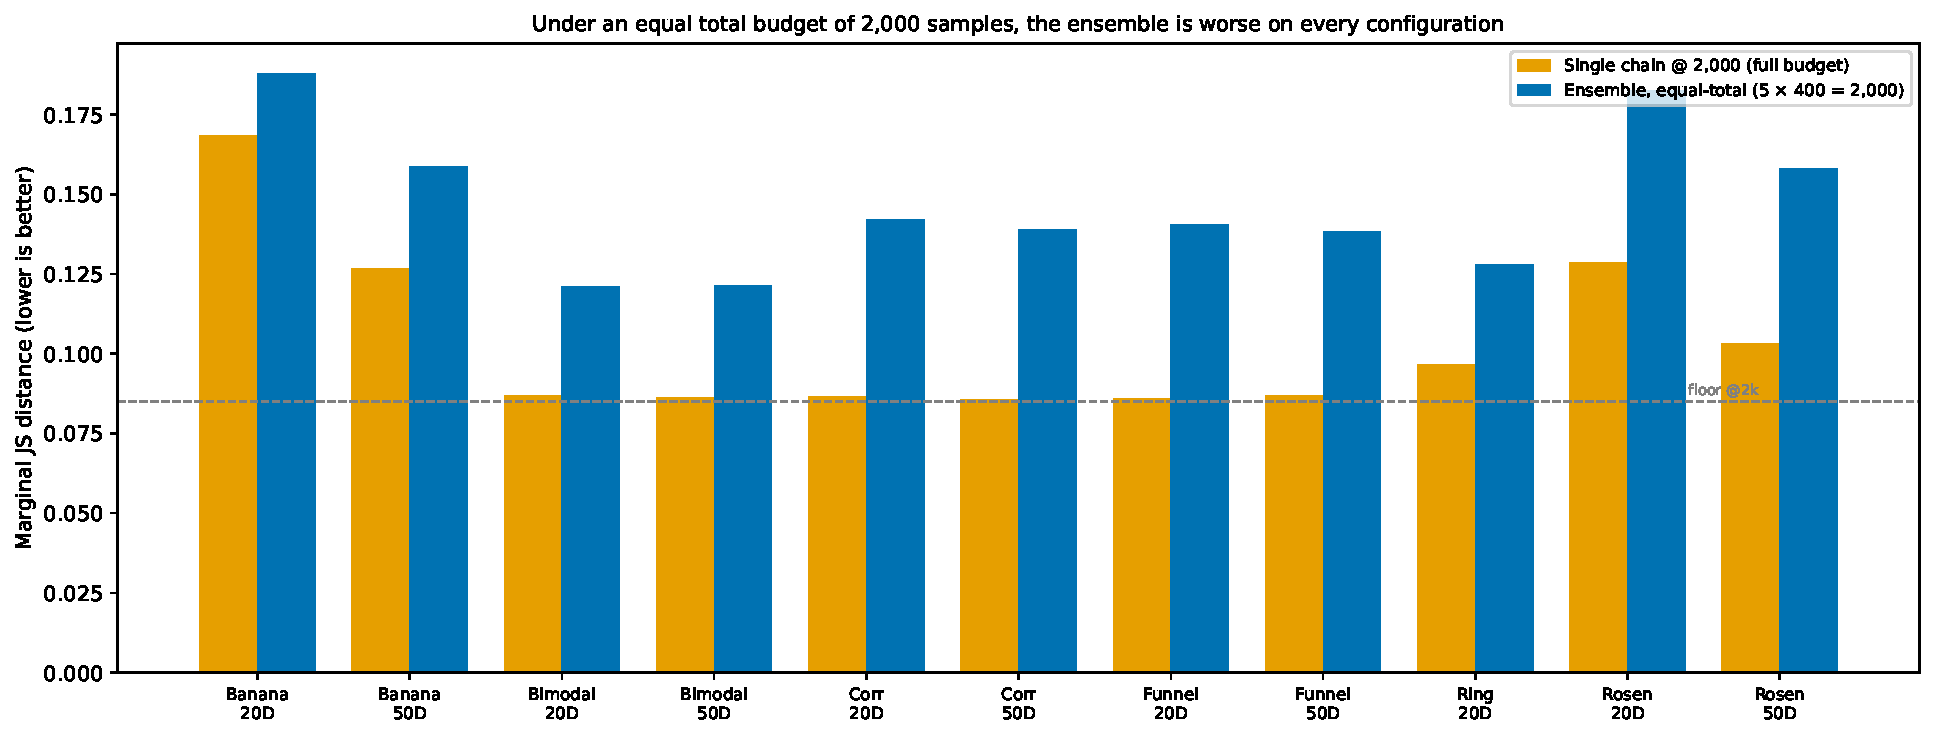
\includegraphics[width=\textwidth]{fig_equal_total.pdf}
\caption{Equal-total budget: with the same 2{,}000-sample total, the ensemble
(five members of 400 samples each) is worse than the single chain on every
configuration, by 11\% to 64\%. The dashed line is the 2{,}000-sample noise
floor.}
\label{fig:equaltotal}
\end{figure}

\subsection{Cost}
\label{sec:cost}
On a single accelerator the equal-per-member ensemble takes about five times
the wall-clock time of the single chain, because it runs five separate flowMC
instances. The cost of one flowMC run is dominated by its fixed training
loops, not by the particle count: on our hardware the 10{,}000-particle chain
runs in about 15 seconds, comparable to the 2{,}000-particle chain (about 18
seconds; the difference is within run-to-run variation) and roughly six times
faster than the ensemble (about 92 seconds). The single chain therefore gets
five times the samples at almost no extra cost, while the ensemble pays a
fivefold cost for samples that are worse. (With five accelerators the members
could run in parallel and the wall-clock would become comparable, but at five
times the hardware and still with worse samples.) In none of our settings is
the ensemble the better choice. Figure~\ref{fig:cost} places the three
samplers on the accuracy--cost plane.

\begin{figure}[htbp]
\centering

\includegraphics[width=0.72\textwidth]{fig_cost.pdf}
\caption{Accuracy versus cost (mean over the eleven configurations; measured
wall-clock runtimes). The equal-budget single chain is simultaneously the most
accurate and the cheapest option, so the ensemble is dominated on both axes:
it costs about six times more and is less accurate.}
\label{fig:cost}
\end{figure}

\section{Discussion}

\subsection{What actually happened}
Several findings point to one conclusion, and the controlled experiments now
say \emph{why}. The ensemble's apparent advantage over a small single chain is
a sample-count artifact whose size is given in closed form by
Equation~\eqref{eq:floor} (Section~\ref{sec:why}); at an equal total budget a
single chain is better (Sections~\ref{sec:control} and~\ref{sec:equaltotal});
member diversity does nothing (Section~\ref{sec:ablation}); and none of the
aggregation heuristics helps (Section~\ref{sec:ablation}). The direct control
in Section~\ref{sec:localize} locates the cause --- replacing the aggregation
with plain uniform pooling returns the accuracy to the single-chain level ---
and the sampler-free decomposition in Section~\ref{sec:decomp} identifies the
mechanism. The deficit has two parts. The resampling-with-replacement step
duplicates points and thereby doubles the sampler-side variance term of the
histogram, an estimator-level loss worth about half of the effective sample,
predicted quantitatively by the bootstrap factor in
Equation~\eqref{eq:floor} and invisible to an unbiased joint metric. The
coverage reweighting (and the tempering schedule, which on healthy members
only ever sharpens the target, up to $\pi^{1.23}$) genuinely distorts the
sampled law, which the energy distance confirms and which is worst exactly
where the cluster structure of the first two coordinates is unbalanced.
Applied to exact samples, the two effects reproduce about 90\% of the measured
ensemble deficit, and with tempering included they reproduce the measured
ensemble values on the correlated and funnel targets nearly exactly. The
sample-set ESS stays near nominal throughout (9{,}848 against 9{,}846 on
exact samples), so this diagnostic cannot detect either effect. A uniform pool
imposes neither, which is why it matches the single chain under this
marginal-JS evaluation.

The real-posterior experiment of Section~\ref{sec:realpost} both extends and
sharpens this picture. On genuine Bayesian posteriors sampled by the real flowMC
kernel, the two conclusions that matter for practice hold under unbiased joint
metrics and not merely under the biased marginal JS: the single chain at the
full budget beats the small one, and the uniform pool is closest to the true
posterior on every metric and every target. The one part of the synthetic story
that does not carry over verbatim is instructive rather than awkward. The full
aggregation stack, which the marginal-JS view condemns, is often the
\emph{best} variant under the energy distance and $\mathrm{MMD}^2$ on these
posteriors, because its damage --- as Section~\ref{sec:decomp} established --- is
concentrated in the resampling step, which distorts a finite-sample-biased
histogram estimator without moving the joint law that an unbiased metric sees.
That the ranking of the aggregation flips exactly between the biased and the
unbiased metric is not a contradiction; it is the clearest possible
confirmation of this paper's central methodological claim, that the verdict of a
sampler comparison is inseparable from the properties of the metric used to
reach it. We therefore state the aggregation result in its precise, metric-aware
form: reweight-and-resample aggregation reliably harms the marginal fit and is
dominated by uniform pooling, while its effect on the joint posterior is small
and occasionally favourable.

Looking back, the part that is a little uncomfortable to admit is how
convincing the wrong version looked. The first draft of this work reported the
18\% improvement with significance on every target and large effect sizes, and
all of that was technically correct --- it just answered the wrong question.
The lesson we take from it is mundane but easy to forget under the pressure of
a positive result: before believing a comparison, make the baselines spend the
same budget.

\subsection{Implication for practice}
For the targets and budgets we study, the practical advice is the opposite of
the method we set out to build. Given a fixed sampling budget, run one flowMC
chain at the full budget instead of splitting or multiplying it across an
ensemble. If for some reason the members are pooled, pool them uniformly ---
concatenation preserves both the law and the effective sample --- and do not
expect to beat the single chain. Avoid coverage-style reweighting,
diagnostic-driven tempering, and in particular any aggregation that resamples
with replacement, which by itself costs half of the effective sample under
histogram-based metrics. Ensembling in this setting adds compute and
complexity and gives nothing back. Three further guidelines concern evaluation
rather than sampling. When a histogram-based divergence such as marginal JS is
used to compare samplers, the comparison is only meaningful at matched sample
counts, and reporting the finite-sample floor of
Equation~\eqref{eq:floor} alongside the results makes the remaining headroom
visible at a glance. Pairing the histogram divergence with an unbiased joint
metric such as the energy distance separates true distributional error from
estimator artifacts, as it did here. And the reference generator itself should
be validated against the potential with an exact-draw test
(Section~\ref{sec:audit}) before any divergence-to-reference number is
interpreted as sampler error.

\subsection{Scope and limitations}
Our headline comparisons concern marginal JS distance on these synthetic
targets. We measured the joint-distribution behaviour of the aggregation
operators with the energy distance, but only on exact samples
(Section~\ref{sec:decomp}); a joint metric evaluated on the actual flowMC
outputs could still reveal mode-coverage effects of ensembling that marginal
JS cannot, and remains the natural way to settle whether ensembling helps for
genuinely two-dimensional multimodal structure. This caveat is not the same
for every target: for the bimodal Gaussian, whose modes are separated along a
single axis, the marginal JS on that axis does reflect mode coverage, so our
conclusion there is on firmer ground; for the Gaussian ring the marginals are
partly washed out, and the audit of Section~\ref{sec:audit} additionally
shows that the ring's released reference differs from its potential, so the
single-chain result on the ring should be read as a statement about marginal
accuracy against that reference. We used the aggregation mechanisms at fixed
default hyperparameters without per-target tuning; tuning might change their
contribution, but a mechanism that has to be tuned carefully just to avoid
harming the result is of limited practical value, and the exact-sample
decomposition shows that two of the three mechanisms (and the shared
resampling step) are harmful at these defaults even under ideal conditions.
The tempering isolation of Section~\ref{sec:decomp} is exact only for the two
target families whose tempered laws are available in closed form. Finally, we
tested six synthetic targets at 20 and 50 dimensions, one flow family, and
ensemble sizes up to twenty members only in the exact-sample setting; real
posteriors, other flows, or other aggregation designs may behave differently.
Beyond these caveats, the extensions that would sharpen the picture most are
evaluating joint metrics on the actual flowMC outputs, repeating the study on
real posteriors with funnel-like or multimodal geometry, and re-running the
Rosenbrock and ring rows against corrected references.

\section{Conclusion}
We set out to validate a diversity-enhanced flowMC ensemble, and instead we
found that its apparent benefit was an artifact of comparing at unequal sample
counts --- an artifact whose size is given in closed form by the
finite-sample law of the histogram JS estimator,
$\mathbb{E}[\widehat{\mathrm{JS}}^{\,2}]\approx c\,(1/N+1/M)$. With a matched
10{,}000-sample budget a single flowMC chain matches or beats the full
ensemble on every target --- winning on nine of eleven configurations and
tying on the two banana cases --- and lowers the mean marginal JS distance by
24\%, while running about six times faster. Taking the ensemble apart shows
where the benefit went: diversity does nothing, none of the three aggregation
heuristics helps, and replacing the aggregation with plain uniform pooling
recovers the single-chain accuracy. Removing flowMC itself then shows why:
applied to exact draws, the aggregation operators reproduce about 90\% of the
deficit, and with the tempering schedule they reproduce the measured ensemble
on the correlated and funnel targets. The damage is the sum of a genuine
distribution shift from the coverage and tempering reweighting --- confirmed
by an unbiased energy distance --- and an estimator-level loss from resampling
with replacement, which halves the effective histogram sample; neither is
visible to the sample-set ESS, and neither is repaired by adding members. An
audit of the reference generators adds a final caution: two of the six targets
were scored against a law that differs from their potential, and once this is
accounted for, only the banana remains genuinely sampler-limited. The
recommendation is short: run one flowMC chain at the full budget; if you pool
members, pool them uniformly --- on the synthetic targets this matches the
single chain, and on the real posteriors it was closest to the truth under
every metric; stay away
from the resampling-and-reweighting machinery; and when benchmarking with a
histogram divergence, match the sample counts, report the floor, validate the
reference, and keep an unbiased joint metric alongside. The broad lesson is an
old one that still catches us: an ensemble compared against a smaller baseline
can look effective for reasons that have nothing to do with the ensemble. The
remedy is equally simple: match the budgets, know the finite-sample floor of
the metric, and give a plain control the chance to falsify the method early.

\section*{Reproducibility}
All target definitions, member configurations, per-repetition seeds, the
control scripts (single at 10{,}000, the homogeneous ensemble, and the
uniform-pooling control) and the analysis code are available at [13]. Every
number reported here can be regenerated from the released seeds. The
repository also includes the CSV outputs used to produce
Tables~\ref{tab:control}--\ref{tab:rawpool} and the corresponding figures.
The sampler-free experiments of Sections~\ref{sec:why},~\ref{sec:decomp}
and~\ref{sec:audit} are produced by a self-contained script
(\texttt{supp\_experiments.py}) that ports the released JS estimator,
aggregation operators and reference generators to NumPy (the ports are checked
for numerical equivalence against the released implementations), together with
its CSV outputs (\texttt{supp\_*.csv}) and the figure-generation code; the
table bodies of this paper are generated directly from the CSVs.

\begin{thebibliography}{99}
\bibitem{wong2023} K.~W.~K. Wong, M.~Gabri\'e, D.~Foreman-Mackey. flowMC:
Normalizing flow enhanced sampling package for probabilistic inference in JAX.
\textit{Journal of Open Source Software}, 8(83):5021, 2023.
\bibitem{gabrie2022} M.~Gabri\'e, G.~M. Rotskoff, E.~Vanden-Eijnden. Adaptive
Monte Carlo augmented with normalizing flows. \textit{PNAS},
119(10):e2109420119, 2022.
\bibitem{papamakarios2021} G.~Papamakarios, E.~Nalisnick, D.~J. Rezende,
S.~Mohamed, B.~Lakshminarayanan. Normalizing Flows for Probabilistic Modeling
and Inference. \textit{JMLR}, 22(57):1--64, 2021.
\bibitem{durkan2019} C.~Durkan, A.~Bekasov, I.~Murray, G.~Papamakarios. Neural
Spline Flows. \textit{NeurIPS 32}, 7509--7520, 2019.
\bibitem{brooks2011} S.~Brooks, A.~Gelman, G.~L. Jones, X.-L. Meng (eds.).
\textit{Handbook of Markov Chain Monte Carlo}. Chapman \& Hall/CRC, 2011.
\bibitem{goodman2010} J.~Goodman, J.~Weare. Ensemble samplers with affine
invariance. \textit{Comm.\ App.\ Math.\ Comp.\ Sci.}, 5(1):65--80, 2010.
\bibitem{emcee2013} D.~Foreman-Mackey, D.~W. Hogg, D.~Lang, J.~Goodman. emcee:
The MCMC Hammer. \textit{PASP}, 125(925):306--312, 2013.
\bibitem{earl2005} D.~J. Earl, M.~W. Deem. Parallel tempering: Theory,
applications, and new perspectives. \textit{Phys.\ Chem.\ Chem.\ Phys.},
7(23):3910--3916, 2005.
\bibitem{neal1996} R.~M. Neal. Sampling from multimodal distributions using
tempered transitions. \textit{Statistics and Computing}, 6(4):353--366, 1996.
\bibitem{neal2003} R.~M. Neal. Slice sampling. \textit{The Annals of
Statistics}, 31(3):705--767, 2003.
\bibitem{lin1991} J.~Lin. Divergence measures based on the Shannon entropy.
\textit{IEEE Trans.\ Inf.\ Theory}, 37(1):145--151, 1991.
\bibitem{geyer1992} C.~J. Geyer. Practical Markov Chain Monte Carlo.
\textit{Statistical Science}, 7(4):473--483, 1992.
\bibitem{repo} M.~Shi. flowmc-ensemble: code and reproducibility artifacts.
GitHub, \url{https://github.com/mingyus3/flowmc-ensemble}, 2025.
\bibitem{miller1955} G.~A. Miller. Note on the bias of information estimates.
In \textit{Information Theory in Psychology: Problems and Methods}, 95--100.
Free Press, 1955.
\bibitem{paninski2003} L.~Paninski. Estimation of entropy and mutual
information. \textit{Neural Computation}, 15(6):1191--1253, 2003.
\bibitem{szekely2013} G.~J. Sz\'ekely, M.~L. Rizzo. Energy statistics: A class
of statistics based on distances. \textit{Journal of Statistical Planning and
Inference}, 143(8):1249--1272, 2013.
\bibitem{gretton2012} A.~Gretton, K.~M. Borgwardt, M.~J. Rasch,
B.~Sch\"olkopf, A.~Smola. A kernel two-sample test. \textit{JMLR},
13:723--773, 2012.
\bibitem{efron1979} B.~Efron. Bootstrap methods: Another look at the
jackknife. \textit{The Annals of Statistics}, 7(1):1--26, 1979.
\end{thebibliography}

\end{document}
